\section{Fonction logarithme népérien}

\subsection{Introduction et définition}

\subsubsection{Introduction}

\begin{tabular}{lllll}
Soit la fonction & $\mathrm{exp} \; \; \; :$ & $\R$ & $\longrightarrow$ & $R$ \\
& & $x$ & $\longmapsto$ & $exp(x) = e^x$ \\
\end{tabular}

On sait que la fonction exponentielle est continue, dérivable et strictement croissante sur $\R$. \\ On sait que pour tout $x \in \R, e^x > 0$. \\

\begin{tikzpicture}[line cap=round,line join=round,>=triangle 45,x=1.0cm,y=1.0cm]
\draw[->] (-2.04,0) -- (2.64,0);
\foreach \x in {-2,-1,1,2}
\draw[shift={(\x,0)}] (0pt,2pt) -- (0pt,-2pt) node[below] {\footnotesize $\x$};
\draw[->] (0,-0.9) -- (0,4.54);
\foreach \y in {,1,2,3,4}
\draw[shift={(0,\y)}] (2pt,0pt) -- (-2pt,0pt) node[left] {\footnotesize $\y$};

\draw[shift={(0,e)}] (2pt,0pt) -- (-2pt,0pt) node[left] {\footnotesize $e$};
\draw (0pt,-10pt) node[right] {\footnotesize $0$};

\clip (-2,-1) rectangle (2.5,4.5);

\draw [domain=-2:3,DarkGreen,smooth,samples=100] plot(\x,{exp(\x*ln(e))}) ;
\draw  (1,2.72)-- ++(-1.5pt,-1.5pt) -- ++(3.0pt,3.0pt) ++(-3.0pt,0) -- ++(3.0pt,-3.0pt);
\draw  (0,2.72)-- ++(-1.5pt,0 pt) -- ++(3.0pt,0 pt) ++(-1.5pt,-1.5pt) -- ++(0 pt,3.0pt);

\begin{pgfonlayer}{background}   
\draw[step=1mm,ultra thin,AntiqueWhite!10] (-2,-1) grid (2.5,4.5);
\draw[step=5mm,very thin,AntiqueWhite!30]  (-2,-1) grid (2.5,4.5);
\draw[step=1cm,very thin,AntiqueWhite!50]  (-2,-1) grid (2.5,4.5);
\draw[step=5cm,thin,AntiqueWhite]          (-2,-1) grid (2.5,4.5);
\end{pgfonlayer}
\end{tikzpicture}


Soit $k > 0$. \\ $k$ a un et un seul antécédent dans $\R$. Donc l'équation $e^x = k$ admet une et une seule solution dans $\R$. \\ 
On note cette solution $\ln k$, et on lit « l n de $k$» cette solution, appelée \textbf{logarithme népérien de k}. \\

\textbf{Exemples} \\

\begin{itemize}
\item[•] $k = 1$ : $1$ a un et un seul antécédent dans $\R$, c'est-à-dire que l'équation $e^x = 1$ admet une solution et une seule dans $\R$ : $0$. \\ Donc $\ln 1 = 0$. \\
\item[•] $k = e$ : $e$ a un et un seul antécédent dans $\R$, c'est-à-dire que l'équation $e^x = e$ admet une solution et une seule dans $\R$ : $1$. \\ Donc $\ln e = 1$.
\end{itemize}

\vspace*{.3cm}

On conclut que pour tout $x \in \R$ et pour tout $k > 0$, $e^x = k \Longleftrightarrow \ln k$ 

\subsubsection{Définition}

La fonction logarithme népérien est la fonction définie sur $\left] 0 \; ; \; +\infty \right[$ qui a tout nombre réel $k$ strictement positif associe l'unique antécédent de $k$ par la fonction exponentielle. \\

\begin{tabular}{llll}
$\ln :$ & $\R$ & $\longrightarrow$ & $\R$ \\
& $k$ & $\longmapsto$ & $\ln k$ \\
\end{tabular}

\vspace*{.3cm}

\begin{tabular}{llll}
On peut étendre cette définition et définir la fonction  $\ln :$ & $\R$ & $\longrightarrow$ & $\R$ \\
& $x$ & $\longmapsto$ & $\ln x$ \\
\end{tabular}

\subsubsection{Conséquence immédiate de la définition}

\begin{tabular}{llll}
Soit la fonction  $\ln :$ & $\R$ & $\longrightarrow$ & $\R$ \\
& $x$ & $\longmapsto$ & $\ln x$ \\
\end{tabular}

On a $D_{\ln} = \left]0 \; ; \; +\infty\right[$. \\

\textbf{Attention !} La notion de $x$ n'a de sens que si $x > 0$. \\

On a : \\

\begin{itemize}
\item[•] $\forall x > 0$, $\forall y \in \R$, $y = \ln x \Longleftrightarrow x = e^y$ \\
\item[•] $\forall x \in \R$, $\forall y > 0$, $y = e^x \Longleftrightarrow x = \ln y$ \\
\item[•] $\forall x > 0$,$ e^{\ln x} = x$ \\
\item[•] $\forall x \in \R$, $\ln\left(e^x\right) = x$ \\
\end{itemize}

\vspace*{.3cm}

De plus : \\

\begin{itemize}
\item[•] $\ln 1 = 0$ \\
\item[•] $\ln e = 1$ \\
\end{itemize}

\subsection{Propriétés fondamentales de la fonction logarithme népérien}

\subsubsection{Relation fonctionnelle}

$\forall a >0$, $\forall b > 0$, $\ln \left(ab\right) = \ln a + \ln b$ \\

\textbf{Démonstration} \\

D'après la définition, $e^{\ln x} = x$. \\

On sait que : $\forall x \in \R$, $\forall y \in \R$, $e^{x+y} = e^x \times e^y$ \\

On a $e^{\ln\left(ab\right)} = ab$ \\

On a aussi $e^{\ln a + \ln b} = e^{\ln a} \times e^{\ln b} = ab$. \\

D'où $e^{\ln\left(ab\right)} = e^{\ln a + \ln b}$. \\

On en conclut que $\ln\left(ab\right) = \ln a + \ln b$. 

\newpage

\subsubsection{Conséquences}

Soient $a>0$ et $b>0$. \\

\begin{itemize}
\item[•] Le logarithme de l'inverse est l'opposé du logarithme : $\ln \dfrac{1}{a} = -\ln a$ \\
\end{itemize}

\textbf{Démonstration} : On a : $e^{\ln \frac{1}{a}} = \dfrac{1}{a}$. On a aussi $e^{-\ln a} = \dfrac{1}{e^{\ln a}} = \dfrac{1}{a}$. \\

Il vient que $e^{\ln \frac{1}{a}} = e^{-\ln a}$. \\

D'où $\ln \dfrac{1}{a} = -\ln a$ \\

\begin{itemize}
\item[•] Le logarithme d'un quotient est la différence des logarithmes : $\ln \dfrac{a}{b} = \ln a - \ln b$ \\
\end{itemize}

\textbf{Démonstration} : $\ln \dfrac{a}{b} = \ln\left(a\times\dfrac{1}{b}\right) = \ln a + \ln \dfrac{1}{b} = \ln a - \ln b$ \\

\begin{itemize}
\item[•] Le logarithme d'un carré est le double du logarithme  : $\ln \left(a^2\right) = 2\ln a$ \\
\end{itemize}

\textbf{Démonstration} : $\ln\left(a^2\right) = \ln\left(a\times a\right) = \ln a + \ln a = 2\ln a$ \\

\begin{itemize}
\item[•] Le logarithme d'une racine carrée est la moitié du logarithme : $\ln \sqrt{a} = \dfrac{1}{2}\ln a$ \\
\end{itemize}

\textbf{Démonstration} : On a $\ln \left[\left(\sqrt{a}\right)^2\right] = 2\ln \sqrt{a}$. On a aussi $\ln \left[\left(\sqrt{a}\right)^2\right] = \ln a$. \\

D'où $2\ln \sqrt{a} = \ln a$ et $\ln \sqrt{a} = \dfrac{1}{2} \ln a$. \\

On a aussi : $\forall n \in \N, \ln \left(a^n\right) = n\ln a$. \\

On a même : $\forall p \in \Z, \ln \left(a^p\right) = p\ln a$. \\

\textbf{Par exemple} : $\ln \left(a^{-2}\right) = \ln \dfrac{1}{a^2} = -\ln\left(a^2\right) = -2\ln a$. \\

On a bien $p = -2$. D'où $\ln\left(a^{-2}\right) = -2\ln a$

\subsubsection{Exemples de calculs}

Exprimer en fonction de $\ln 3$.  \\

\begin{tabular}{lll}

\begin{minipage}{7cm}
\vspace*{-.6cm}
\begin{tabular}{lll}
$A$ & $ = $ & $ \ln 27$ \\
$A$ & $=$ & $\ln \left(3^3\right)$ \\
$A$ & $=$ & $3\ln 3$ \\
\end{tabular}
\end{minipage}

&

\begin{minipage}{7cm}
\hspace*{-1cm}
\begin{tabular}{lll}
$B$ & $ = $ & $ \ln \dfrac{1}{9}$ \vspace*{.1cm} \\
$B$ & $=$ & $-\ln 9$ \\
$B$ & $=$ & $-\ln \left(3^2\right)$ \\
$B$ & $=$ & $-2\ln 3$ \\
\end{tabular}
\end{minipage}

&

\begin{minipage}{7cm}
\hspace*{-1.5cm}
\begin{tabular}{lll}
$C$ & $ = $ & $ \ln 63 - \ln 7 $ \\
$C$ & $=$ & $ \ln \dfrac{63}{7} $ \vspace*{.1cm} \\
$C$ & $=$ & $ \ln 9 $ \\
$C$ & $=$ & $ \ln \left(3^2\right) $ \\
$C$ & $=$ & $ 2\ln 3 $ \\
\end{tabular}
\end{minipage}

\\

\begin{minipage}{7cm}
\vspace*{.3cm}
\begin{tabular}{lll}
$D$ & $ = $ & $ 4\ln 6 - \ln 16 $ \\
$D$ & $=$ & $ \ln \left(6^4\right) - \ln 16 $ \\
$D$ & $=$ & $ \ln 1296 - \ln 16 $ \vspace*{.1cm} \\
$D$ & $=$ & $ \ln \dfrac{1296}{16} $ \vspace*{.1cm} \\
$D$ & $=$ & $ \ln 81 $ \\
$D$ & $=$ & $ \ln \left(3^4\right) $ \\
$D$ & $=$ & $ 4\ln 3 $ \\
\end{tabular} 
\end{minipage}

\\

\end{tabular}

\vspace*{-5cm}

\newpage

\subsection{Dérivée de la fonction logarithme népérien}

\begin{tabular}{llll}
Soit la fonction  $\ln :$ & $\R$ & $\longrightarrow$ & $\R$ \\
& $x$ & $\longmapsto$ & $\ln x$ \\
\end{tabular}

\vspace*{.3cm}

On a $D_{\ln} = \R^+* = \left] 0 \; ; \; +\infty\right[$. \\

La fonction $\ln$ est dérivable sur $\left] 0 \; ; \; +\infty\right[$ et pour tout $x \in \left] 0 \; ; \; +\infty\right[$, $\ln'x = \dfrac{1}{x}$. \\

\textbf{Démonstration} : \\

\begin{tabular}{llll}
Soit la fonction  $f :$ & $\R$ & $\longrightarrow$ & $\R$ \\
& $x$ & $\longmapsto$ & $f(x) = e^{\ln x}$ \\
\end{tabular}

\vspace*{.3cm}

$D_f = \left] 0 \; ; \; +\infty\right[$. \\

On pose $u(x) = \ln x$. \\

On sait que $\left(e^u\right)' = u'e^u$. D'où $f'(x) = \left(\ln'x\right)e^{\ln x}$. \\

Or, on sait que $e^{\ln x} = x$. \\

D'où $f'(x) = \left(\ln'x\right)x$. \\

Cependant, $\forall x \in \left] 0 \; ; \; +\infty\right[, f(x) = x$ et $f'(x) = 1$. \\

D'où $\left(\ln'x\right)x = 1$ et $\ln'x = \dfrac{1}{x}$. 

\subsection{Étude de la fonction logarithme népérien}

\begin{tabular}{llll}
Soit la fonction  $\ln :$ & $\R$ & $\longrightarrow$ & $\R$ \\
& $x$ & $\longmapsto$ & $\ln x$ \\
\end{tabular}

\begin{itemize}
\item[•] On a $D_{\ln} = \left]0 \; ; \; +\infty\right[$. \\

\item[•] On étudie les variations de $\ln$. \\
\end{itemize}

On a $\ln'x = \dfrac{1}{x}$, et $\forall x \in \R, \dfrac{1}{x} > 0$. \\

Donc $\ln'x >0$, on en déduit le tableau de variations suivant : \\

\variations
x & -\infty & & 0 & & & & +\infty \\
\ln'x & \ha & \ha & \bb & & + & & & \\
\ln x & \hv & \hv & \bb & \b\mI & \cl & & \h\pI \\
\fin

\vspace*{.3cm}

On a $ \displaystyle {\lim_{x \rightarrow -\infty}} \; e^x = 0$, d'où $ \displaystyle {\lim_{x \rightarrow 0^+}} \; \ln x = -\infty$. \\

On a aussi  $ \displaystyle {\lim_{x \rightarrow +\infty}} \; e^x = +\infty$, d'où $ \displaystyle {\lim_{x \rightarrow +\infty}} \; \ln x = +\infty$.

\newpage

\vspace*{-1.2cm}

\begin{itemize}
\item[•] On étudie la dérivée seconde de la fonction $\ln$
\end{itemize}

\vspace*{.3cm}

$\ln''x = \left(\dfrac{1}{x}\right)' = \dfrac{-1}{x^2}$. \\

Or, pour tout $x \in \R, x^2 \geqslant 0$, donc $\dfrac{-1}{x^2} < 0$. \\

On a $\ln''x < 0$, on peut en déduire la propriété suivante : \\

\variations
x & -\infty & & 0 & & & & +\infty \\
\ln''x & \ha & \ha & \bb & & \; \; \; \; \; \; \; \; \; \; \; \; \; \; \;  - &  & & \\
\ln x & \hv & \hv & \bb & \mathrm{La} & \mathrm{fonction \ln } & \mathrm{est} & \mathrm{concave} \\
\fin

\vspace*{.3cm}

\begin{itemize}
\item[•] On étudie la représentation graphique de la fonction $\ln$
\end{itemize}

\vspace*{.3cm}

\begin{tabular}{ll}
\begin{minipage}{12cm}

\begin{tikzpicture}[line cap=round,line join=round,>=triangle 45,x=1.0cm,y=1.0cm]
\draw[->] (-1.72,0) -- (9.46,0);
\foreach \x in {-1,1,2,e,3,4,5,6,7,e^2,8,9}
\draw[shift={(\x,0)}] (0pt,2pt) -- (0pt,-2pt) node[below] {\footnotesize $\x$};

\draw[->] (0,-1.97) -- (0,3.24);
\foreach \y in {-1,1,2,3}
\draw[shift={(0,\y)}] (2pt,0pt) -- (-2pt,0pt) node[left] {\footnotesize $\y$};
\draw (0pt,-8pt) node[left] {\footnotesize $0$};

\clip(-1.7,-1.9) rectangle (9.5,3.25);
\draw[color=blue,smooth,samples=100,domain=.01:9] plot(\x,{ln((\x))});
\draw[color=green,smooth,samples=100,domain=-1.5:2.8] plot(\x,{(\x)-1});
\draw [<->, green] (0.69,-0.31) -- (1.31,0.31);
\draw [<->, green] (2.14,0.79) -- (3.34,1.23);
\draw[dashed] (0,1) -- (  e,1) -- (  e,0) ; 
\draw[dashed] (0,2) -- (e*e,2) -- (e*e,0) ; 


\draw [color=blue] (1,0)-- ++(-1.5pt,-1.5pt) -- ++(3.0pt,3.0pt) ++(-3.0pt,0) -- ++(3.0pt,-3.0pt);
\draw[color=blue] (0.84,0.37) node {$A$};
\draw [color=blue] (2.72,1)-- ++(-1.5pt,-1.5pt) -- ++(3.0pt,3.0pt) ++(-3.0pt,0) -- ++(3.0pt,-3.0pt);
\draw[color=blue] (2.86,1.28) node {$B$};
\draw [color=blue] (7.39,2)-- ++(-1.5pt,-1.5pt) -- ++(3.0pt,3.0pt) ++(-3.0pt,0) -- ++(3.0pt,-3.0pt);

\begin{pgfonlayer}{background}   
\draw[step=1mm,ultra thin,AntiqueWhite!10] (-1.7,-1.9) grid (9.5,3.25);
\draw[step=5mm,very thin,AntiqueWhite!30]  (-1.7,-1.9) grid (9.5,3.25);
\draw[step=1cm,very thin,AntiqueWhite!50]  (-1.7,-1.9) grid (9.5,3.25);
\draw[step=5cm,thin,AntiqueWhite]          (-1.7,-1.9) grid (9.5,3.25);
\end{pgfonlayer}


\end{tikzpicture}
\end{minipage}
&
\begin{minipage}{5cm}
On a $\ln 1 = 0$ car $e^0 = 1$. \\
On a aussi $\ln e = 1$ car $e^1 = e$. 
\end{minipage}
\end{tabular}

\vspace*{.3cm}

\begin{itemize}
\item[•] On étudie l'équation de la tangente à la courbe au point $A\left(1\; ; \; 0\right)$.
\end{itemize}

\vspace*{.3cm}

\begin{tabular}{lll}
$y$ & $=$ & $\ln'1\left(x-1\right)+\ln 1$ \vspace*{.2cm} \\
$y$ & $=$ & $\dfrac{1}{1}\left(x-1\right)+0$ \vspace*{.2cm} \\
$y$ & $=$ & $x-1$
\end{tabular}

\vspace*{.3cm}

\begin{itemize}
\item[•] On étudie l'équation de la tangente à la courbe au point $B\left(e\; ; \; 1\right)$.
\end{itemize}

\vspace*{.3cm}

\begin{tabular}{lll}
$y$ & $=$ & $\ln'e\left(x-e\right)+\ln e$ \vspace*{.2cm} \\
$y$ & $=$ & $\dfrac{1}{e}\left(x-e\right)+1$ \vspace*{.2cm} \\
$y$ & $=$ & $\dfrac{1}{e} \times x - \dfrac{e}{e} + 1$ \vspace*{.2cm} \\
$y$ & $=$ & $\dfrac{1}{e}x - 1 + 1$ \vspace*{.2cm} \\
$y$ & $=$ & $\dfrac{1}{e}x$ \vspace*{.2cm} \\
\end{tabular}

\vspace*{.3cm}

\begin{itemize}
\item[•] On étudie le signe de $\ln x$. \\

\begin{itemize}
\item[*] Pour $0 < x < 1$, $\ln x < 0$.
\item[*] Pour $x = 1$, $\ln x = 0$.
\item[*] Pour $x > 1$, $\ln x > 0$.
\end{itemize}
\end{itemize}

\vspace*{-5cm}

\newpage

\vspace*{-1.8cm}

\subsection{Comparaison des fonctions logarithme népérien et exponentielle}

\begin{tikzpicture}[line cap=round,line join=round,>=triangle 45,x=1.0cm,y=1.0cm, scale=.8]
\draw [red,line width=1.6pt] (-5,0) -- (8.5,0);
\draw[->] (-5.5,0) -- (9.2,0);
\foreach \x in {-5,...,9}
\draw[shift={(\x,0)}] (0pt,2pt) -- (0pt,-2pt) node[below] {\footnotesize $\x$};
\draw[shift={(e,0)}] (0pt,2pt) -- (0pt,-2pt) node[below] {\tiny $e$};

\draw [red,line width=1.6pt] (0,-4) -- (0,4.75);
\draw[->] (0,-5) -- (0,5.2);
\foreach \y in {-5,...,5}
\draw[shift={(0,\y)}] (2pt,0pt) -- (-2pt,0pt) node[left] {\footnotesize $\y$};
\draw[shift={(0,e)}] (2pt,0pt) -- (-2pt,0pt) node[left] {\footnotesize $e$};

\draw (0pt,-10pt) node[right] {\footnotesize $0$};

\clip(-5.5,-5.5) rectangle (9.5,5.5);
\draw[green,smooth,samples=100,domain=.01:9] plot(\x,{ln((\x))});
\draw [green] (8,{ln(8)}) node [above] {$y=\ln x$} ;
\draw[red,smooth,samples=100,domain=-6:3] plot(\x,{exp(\x*ln(e))}) ;
\draw [red] (1.5,{exp(1.5*ln(e))}) node [right] {$y=e^x$} ;
\draw[dashdotted,line width=1.2pt, smooth,samples=100,domain=-6:6] plot(\x,\x);
\draw  (4.5,4.25) node [right] {$y=x$} ;

\draw [<->, blue] (0.69,-0.31) -- (1.31,0.31);
\draw [<->, blue] (2.14,0.79) -- (3.34,1.23);
\draw[dashed] (0,1) -- (  e,1) -- (  e,0) ; 
\draw[dashed] (0,2) -- (e*e,2) -- (e*e,0) ; 
\draw[dashed] (0,e) -- (1,e) -- (1,0) ; 
\draw [<->, blue] (-0.31,0.69) -- (0.31,1.31);
\draw [<->, blue] (0.79,2.14) -- (1.23,3.34);



\draw [color=blue] (1,0)-- ++(-1.5pt,-1.5pt) -- ++(3.0pt,3.0pt) ++(-3.0pt,0) -- ++(3.0pt,-3.0pt);
%\draw[color=blue] (0.84,0.37) node {$A$};
\draw [color=blue] (e,1)-- ++(-1.5pt,-1.5pt) -- ++(3.0pt,3.0pt) ++(-3.0pt,0) -- ++(3.0pt,-3.0pt);
%\draw[color=blue] (2.86,1.28) node {$B$};
\draw [color=blue] (e*e,2)-- ++(-1.5pt,-1.5pt) -- ++(3.0pt,3.0pt) ++(-3.0pt,0) -- ++(3.0pt,-3.0pt);

\draw [color=blue] (0,1)-- ++(-1.5pt,-1.5pt) -- ++(3.0pt,3.0pt) ++(-3.0pt,0) -- ++(3.0pt,-3.0pt);
\draw [color=blue] (1,e)-- ++(-1.5pt,-1.5pt) -- ++(3.0pt,3.0pt) ++(-3.0pt,0) -- ++(3.0pt,-3.0pt);

\begin{pgfonlayer}{background}   
\draw[step=1mm,ultra thin,AntiqueWhite!10] (-5.5,-5.5) grid (9.5,5.5);
\draw[step=5mm,very thin,AntiqueWhite!30]  (-5.5,-5.5) grid (9.5,5.5);
\draw[step=1cm,very thin,AntiqueWhite!50]  (-5.5,-5.5) grid (9.5,5.5);
\draw[step=5cm,thin,AntiqueWhite]          (-5.5,-5.5) grid (9.5,5.5);
\end{pgfonlayer}

\end{tikzpicture}

\vspace*{.3cm}

Les deux courbes sont symétriques par rapport à la droite d'équation $y = x$. \\

On a : $\forall x \in \left] 0 \; ; \; +\infty\right[, \ln x < x < e^x$.

\subsection{Étude de fonctions comportant des logarithmes}

\subsubsection{Étude \no 1}

\begin{tabular}{llll}
Soit la fonction  $f :$ & $\R$ & $\longrightarrow$ & $\R$ \\
& $x$ & $\longmapsto$ & $f\left(x\right) = x + \ln x$ \\
\end{tabular}

\begin{itemize}
\item[•] On a $D_{f} = \left]0 \; ; \; +\infty\right[$. 

\item[•] On étudie les variations de $f$. \\
\end{itemize}

On a $f'(x) = 1 + \dfrac{1}{x} = \dfrac{x+1}{x}$. \\

\begin{tabular}{lll}
On a $f'(x) = 0$ & $\Longleftrightarrow$ & $x + 1 = 0$ \\
& $\Longleftrightarrow$ & $x = -1$ \\
\end{tabular}

Le signe de $f'(x)$ est le signe de $x+1$ car pour tout $x \in D_f, x>0$. \\

\variations
x & -\infty & & -1 & & 0 & & & & & & +\infty \\
x+1 & & - & \z & + & \bb & & & + & & \\
f'(x) & \ha & \ha & \ha & \ha & \bb & & & + & & & \\
f(x) & \hv & \hv & \hv & \hv & \bb & \b\mI & & \cl & & & \h\pI \\
\fin

\vspace*{.3cm}

On a $ \displaystyle {\lim_{x \rightarrow 0^+}} \; \ln x = -\infty$, d'où $ \displaystyle {\lim_{x \rightarrow 0^+}} \; f(x) = -\infty$. 

\vspace*{.2cm}

On a aussi  $ \displaystyle {\lim_{x \rightarrow +\infty}} \; \ln x = +\infty$, d'où $ \displaystyle {\lim_{x \rightarrow +\infty}} \; f(x) = +\infty$. \\

$f$ admet une asymptote verticale d'équation $x = 0$. 

\vspace*{-5cm}

\newpage

\begin{itemize}
\item[•] On étudie la dérivée seconde de la fonction $f$.
\end{itemize}

\vspace*{.3cm}

$\ln''x = \left( 1 + \dfrac{1}{x}\right)' = \dfrac{-1}{x^2}$. \\

Or, pour tout $x \in \R, x^2 \geqslant 0$, donc $\dfrac{-1}{x^2} < 0$. \\

On a $f''(x) < 0$, on peut en déduire la propriété suivante : \\

\variations
x & -\infty & & 0 & & & & +\infty \\
\ln''x & \ha & \ha & \bb & & \; \; \; \; \; \; \; \; \; \; \; \; \; \; \;  - &  & & \\
f(x) & \hv & \hv & \bb & \mathrm{La} & \mathrm{fonction    \; f } & \mathrm{est} & \mathrm{concave} \\
\fin

\vspace*{.3cm}

\begin{itemize}
\item[•] On étudie la représentation graphique de la fonction $f$.
\end{itemize}

%\vspace*{.3cm}

\begin{tikzpicture}[line cap=round,line join=round,>=triangle 45,x=1.0cm,y=1.0cm]
\draw[->] (-1.5,0) -- (5.2,0);
\foreach \x in {-1,1,2,3,4}
\draw[shift={(\x,0)}] (0pt,2pt) -- (0pt,-2pt) node[below] {\footnotesize $\x$};

\draw [red,line width=2pt] (0,-5.5) -- (0,4);
\draw[->] (0,-5) -- (0,5.2);
\foreach \y in {-5,-4,-3,-2,-1,1,2,3,4,5}
\draw[shift={(0,\y)}] (2pt,0pt) -- (-2pt,0pt) node[left] {\footnotesize $\y$};

\draw (0pt,-8pt) node[left] {\footnotesize $0$};

\clip(-2,-5.5) rectangle (5.5,5.5);

\draw[green,smooth,samples=100,domain=.01:9] plot(\x,{(\x)+ln((\x))});
\draw[blue,smooth,samples=100,domain=-1:5] plot(\x,{-1+2*\x}) ;
\draw [blue] (0,-1)-- ++(-1.5pt,-1.5pt) -- ++(3.0pt,3.0pt) ++(-3.0pt,0) -- ++(3.0pt,-3.0pt);
\draw [blue] (1,1)-- ++(-1.5pt,-1.5pt) -- ++(3.0pt,3.0pt) ++(-3.0pt,0) -- ++(3.0pt,-3.0pt);
\draw [blue] (3,{3+ln(3)})-- ++(-1.5pt,-1.5pt) -- ++(3.0pt,3.0pt) ++(-3.0pt,0) -- ++(3.0pt,-3.0pt);
\draw [<->, blue] (0.7,{-1+2*.7}) -- (1.3,{-1+2*1.3});

\begin{pgfonlayer}{background}   
\draw[step=1mm,ultra thin,AntiqueWhite!10] (-2,-5.5) grid (5.5,5.5);
\draw[step=5mm,very thin,AntiqueWhite!30]  (-2,-5.5) grid (5.5,5.5);
\draw[step=1cm,very thin,AntiqueWhite!50]  (-2,-5.5) grid (5.5,5.5);
\draw[step=5cm,thin,AntiqueWhite]          (-2,-5.5) grid (5.5,5.5);
\end{pgfonlayer}

\end{tikzpicture}

\vspace*{.3cm}

\begin{itemize}
\item[•] On étudie l'équation de la tangente à la courbe au point $I\left(1\; ; \; 1\right)$.
\end{itemize}

\vspace*{.3cm}

\begin{tabular}{lll}
$y$ & $=$ & $f'(1)\left(x-1\right)+ f(1)$ \vspace*{.2cm} \\
$y$ & $=$ & $ \left( 1 + \dfrac{1}{1}\right) \left(x-1\right)+ \left(1 + \ln 1\right)$ \vspace*{.2cm} \\
$y$ & $=$ & $2\left(x-1\right) + 1$ \vspace*{.2cm} \\
$y$ & $=$ & $2x +1$ \\
\end{tabular}

\vspace*{-5cm}

\newpage

\vspace*{-2.5cm}

\subsubsection{Étude \no 2}

\begin{tabular}{llll}
Soit la fonction  $f :$ & $\R$ & $\longrightarrow$ & $\R$ \\
& $x$ & $\longmapsto$ & $f\left(x\right) = x - \ln x$ \\
\end{tabular}

\begin{itemize}
\item[•] On a $D_{f} = \left]0 \; ; \; +\infty\right[$. 

\item[•] On étudie les variations de $f$. \\
\end{itemize}

On a $f'(x) = 1 - \dfrac{1}{x} = \dfrac{x-1}{x}$. \\

\begin{tabular}{lll}
On a $f'(x) = 0$ & $\Longleftrightarrow$ & $x - 1 = 0$ \\
& $\Longleftrightarrow$ & $x = 1$ \\
\end{tabular}

Le signe de $f'(x)$ est le signe de $x-1$ car pour tout $x \in D_f, x>0$. \\

\variations
x & -\infty & & 0 & & & & 1 & & +\infty \\
f'(x) & \ha & \ha & \bb & & & - & \z & + & \\
f(x) & \hv & \hv & \bb & \h\pI & & \dl & \b{1} & \cl & \h\pI \\
\fin

\vspace*{.3cm}

On a $ \displaystyle {\lim_{x \rightarrow 0^+}} \; \ln x = -\infty$, d'où $ \displaystyle {\lim_{x \rightarrow 0^+}} \; f(x) = +\infty$. 

\vspace*{.2cm}

On a aussi  $ \displaystyle {\lim_{x \rightarrow +\infty}} \; \ln x = $ forme indéterminée, car $\displaystyle {\lim_{x \rightarrow +\infty}} \; x = + \infty$ et $\displaystyle {\lim_{x \rightarrow +\infty}} \; \ln x = + \infty$ \\

$f$ admet une asymptote verticale d'équation $x = 0$. \\

On a un minimum $m\left(1\; ; \; 1\right)$, donc une tangente horizontale à la courbe au point I d'abscisse 1.  

\vspace*{.3cm}

\begin{itemize}
\item[•] On étudie la dérivée seconde de la fonction $f$.
\end{itemize}

\vspace*{.3cm}

$\ln''x = \left( 1 - \dfrac{1}{x}\right)' = \dfrac{1}{x^2}$. On a $f''(x) > 0$, on peut en déduire la propriété suivante : \\

\variations
x & -\infty & & 0 & & & & +\infty \\
\ln''x & \ha & \ha & \bb & & \; \; \; \; \; \; \; \; \; \; \; \; \; \; \;  - &  & & \\
f(x) & \hv & \hv & \bb & \mathrm{La} & \mathrm{fonction f } & \mathrm{est} & \mathrm{concave} \\
\fin

\vspace*{.3cm}

\begin{itemize}
\item[•] On étudie la représentation graphique de la fonction $f$.
\end{itemize}

\vspace*{.3cm}

\begin{tikzpicture}[line cap=round,line join=round,>=triangle 45,x=1.0cm,y=1.0cm]
\draw[->] (-1.5,0) -- (8.2,0);
\foreach \x in {-1,1,2,3,4,5,6,7,8}
\draw[shift={(\x,0)}] (0pt,2pt) -- (0pt,-2pt) node[below] {\footnotesize $\x$};

\draw [red,line width=2pt] (0,-1.5) -- (0,5.5);
\draw[->] (0,-2) -- (0,5.2);
\foreach \y in {-1,1,2,3,4,5}
\draw[shift={(0,\y)}] (2pt,0pt) -- (-2pt,0pt) node[left] {\footnotesize $\y$};

\draw (0pt,-8pt) node[left] {\footnotesize $0$};

\clip(-2,-1.5) rectangle (9,5.5);

\draw[blue,smooth,samples=100,domain=.01:9] plot(\x,{(\x)-ln((\x))});
\foreach \x in {.5,.75,1,2,4,6,7}
    \draw [blue] (\x,{(\x)-ln((\x))})-- ++(-1.5pt,-1.5pt) -- ++(3.0pt,3.0pt) ++(-3.0pt,0) -- ++(3.0pt,-3.0pt);


\draw [<->, green] (0.5,1) -- (1.5,1);

\begin{pgfonlayer}{background}   
\draw[step=1mm,ultra thin,AntiqueWhite!10] (-2,-1.5) grid (9,5.5);
\draw[step=5mm,very thin,AntiqueWhite!30]  (-2,-1.5) grid (9,5.5);
\draw[step=1cm,very thin,AntiqueWhite!50]  (-2,-1.5) grid (9,5.5);
\draw[step=5cm,thin,AntiqueWhite]          (-2,-1.5) grid (9,5.5);
\end{pgfonlayer}

\end{tikzpicture}

\vspace*{-5cm}

\newpage

\vspace*{-2cm}

\subsubsection{Étude \no 3}

\begin{tabular}{llll}
Soit la fonction  $f :$ & $\R$ & $\longrightarrow$ & $\R$ \\
& $x$ & $\longmapsto$ & $f\left(x\right) = \dfrac{\ln x}{x}$ \\
\end{tabular}

\begin{itemize}
\item[•] On a $D_{f} = \left]0 \; ; \; +\infty\right[$. 

\item[•] On étudie les variations de $f$. \\
\end{itemize}

\begin{tabular}{llll}
On pose & $u(x) = \ln x$ & et & $v(x) = x$ \\
D'où & $u'(x) = \dfrac{1}{x}$ & et & $v'(x) = 1$ \\
\end{tabular}

\vspace*{.3cm}

$f$ est de la forme $f = \dfrac{u}{v}$, d'où $f' = \dfrac{u'v - uv'}{v^2}$. \vspace*{.3cm} \\

\begin{tabular}{llll}
Ainsi $\forall x \in \left]0 \; ; \; +\infty\right[$, & $f'(x)$ & $=$ & $\dfrac{\dfrac{1}{x} \times x - \ln x \times 1}{x^2}$ \vspace*{.3cm} \\
& & $=$ & $\dfrac{\dfrac{x}{x} - \ln x}{x^2}$ \vspace*{.3cm} \\
& & $=$ & $\dfrac{1 - \ln x}{x^2}$ \vspace*{.3cm} \\
\end{tabular}

\begin{tabular}{lll}
On a $f'(x) = 0$ & $\Longleftrightarrow$ & $\dfrac{1-\ln x}{x^2} = 0$ \\
& $\Longleftrightarrow$ & $1 - \ln x = 0$ \\
& $\Longleftrightarrow$ & $\ln x = 1$ \\
& $\Longleftrightarrow$ & $x = e$ \\
\end{tabular}

\vspace*{.3cm}

Le signe de $f'(x)$ est le signe de $1 - \ln x$ car pour tout $x \in D_f, x^2>0$. \\

\begin{tabular}{llll}
On a : & $x<e$ & $\Longleftrightarrow$ & $\ln x < 1$ \\
& & $\Longleftrightarrow$ & $-\ln x > -1$ \\
& & $\Longleftrightarrow$ & $1 - \ln x > 0$ \\
\end{tabular}

\vspace*{.3cm}

\begin{tabular}{llll}
On a aussi : & $x>e$ & $\Longleftrightarrow$ & $\ln x > 1$ \\
& & $\Longleftrightarrow$ & $-\ln x < -1$ \\
& & $\Longleftrightarrow$ & $1 - \ln x < 0$ \\
\end{tabular}

\vspace*{.3cm}

On en déduit le tableau de variations suivant : \\

\variations
x & -\infty & & 0 & & & & e & & +\infty \\
f'(x) & \ha & \ha & \bb & & + & & \z & - & \\
f(x) & \hv & \hv & \bb & \b\mI & \cl & & \h{\dfrac{1}{e}} & \dl & \b{0} \\
\fin

\begin{tabular}{ll}
\hspace*{9.7cm}
&
\begin{minipage}{6.3cm}

\vspace*{-4cm}

$f(e) = \dfrac{\ln e}{e} = \dfrac{1}{e}$ \\ On a $\dfrac{1}{e} \approx 0,37$. \\

La fonction $f$ admet un maximum en $M\left(e\; ; \; \dfrac{1}{e}\right)$, donc une tangente horizontale à la courbe au point $M$ d'abscisse $e$.

\end{minipage}

\end{tabular}

On a $ \displaystyle {\lim_{x \rightarrow 0^+}} \; \ln x = -\infty$ et $ \displaystyle {\lim_{x \rightarrow 0^+}} \; x = 0^+$ d'où $ \displaystyle {\lim_{x \rightarrow 0^+}} \; f(x) = -\infty$. 

\vspace*{.2cm}

On a aussi  $ \displaystyle {\lim_{x \rightarrow +\infty}} \; \ln x = +\infty$ et $ \displaystyle {\lim_{x \rightarrow +\infty}} \; x = +\infty$,  d'où $ \displaystyle {\lim_{x \rightarrow +\infty}} \; f(x) =$ forme indéterminée. \\

Néanmoins, on lit graphiquement que $ \displaystyle {\lim_{x \rightarrow +\infty}} \; f(x) = 0^+$. \\

$f$ admet une asymptote verticale d'équation $x = 0$ et une asymptote horizontale en $y = 0$. 

\vspace*{-5cm}

\newpage

\vspace*{-1.3cm}

\begin{itemize}
\item[•] On étudie la dérivée seconde de la fonction $f$.
\end{itemize}

\vspace*{.3cm}

$f''(x) = \left(\dfrac{1 - \ln x}{x^2}\right)'$. \\

\begin{tabular}{llll}
On pose & $u(x) = 1 - \ln x$ & et & $v(x) = x^2$ \\
D'où & $u'(x) = -\dfrac{1}{x}$ & et & $v'(x) = 2x$ \\
\end{tabular}

\vspace*{.3cm}

\begin{tabular}{llll}
$\forall x \in \left]0 \; ; \; +\infty\right[,$ & $f''(x)$ & $=$ & $\dfrac{-\dfrac{1}{x}\times x^2 - \left(1-\ln x\right)\times 2x}{\left(x^2\right)^2}$ \vspace*{.3cm} \\
& & $=$ & $\dfrac{-x -2x + 2x\ln x}{x^4}$ \vspace*{.3cm} \\
& & $=$ & $\dfrac{2x\ln x - 3x}{x^4}$ \vspace*{.3cm} \\
& & $=$ & $\dfrac{x\left(2\ln x - 3\right)}{x^4}$ \vspace*{.3cm} \\
& & $=$ & $\dfrac{2\ln x - 3}{x^3}$ \\
\end{tabular}

\vspace*{.3cm}

On étudie le signe de $f''(x)$. \\

\begin{tabular}{lll}
On a $2\ln x -3 > 0$ & $\Longleftrightarrow$ & $2 \ln x > 3$ \\
& $\Longleftrightarrow$ & $\ln x > \dfrac{3}{2}$ \\
& $\Longleftrightarrow$ & $x > e^{\frac{3}{2}}$ \\
\end{tabular}

\vspace*{.3cm}

\begin{tabular}{lll}
De même, on a $2\ln x -3 < 0$ & $\Longleftrightarrow$ & $2 \ln x < 3$ \\
& $\Longleftrightarrow$ & $\ln x < \dfrac{3}{2}$ \\
& $\Longleftrightarrow$ & $x < e^{\frac{3}{2}}$ \\
\end{tabular}

\vspace*{.3cm}

On peut donc en déduire le tableau de signes suivant : \\

\begin{tikzpicture}
\tkzTabInit[lgt=5,espcl=3]
{ $x$  /1,
$x^3$  /1,
$2\ln x - 3$ /1,
$f''(x)$ /1}
{$ -\infty $ , $0$ , $e^{\frac{3}{2}}$ , $ +\infty $}
\tkzTabLine{, - , z , + ,  t  , + ,  }
\tkzTabLine{, h , d , - ,  z  , + ,  }
\tkzTabLine{, h , d , - ,  z  , + ,  }
\end{tikzpicture}

\vspace*{.3cm}

On peut en déduire la propriété suivante : \\

\variations
x & -\infty & & 0 & & & e^{\frac{3}{2}} & & +\infty \\
f''(x) & \ha & \ha & \bb & - &  & \z & + & \\
f(x) & \hv & \hv & \bb & \mathrm{la \; fonction \; f \; est \; concave} & & \l & \mathrm{la \; fonction \; f \; est \; convexe} & \\
\fin

\vspace*{.3cm}

Donc le point $I$ d'abscisse $e^{\frac{3}{2}}$ est un point d'inflexion.

\vspace*{-5cm}

\newpage

\begin{itemize}
\item[•] On étudie la représentation graphique de la fonction $f$.
\end{itemize}

\vspace*{.6cm}

\begin{tikzpicture}[line cap=round,line join=round,>=triangle 45,x=1.0cm,y=1.0cm]
\draw[->] (-1.75,0) -- (5.3,0);
\foreach \x in {-1,1,2,e,3,4,5}
\draw[shift={(\x,0)}] (0pt,2pt) -- (0pt,-2pt) node[below] {\footnotesize $\x$};

\draw[->] (0,-3) -- (0,3.25);
\foreach \y in {-1,1/e, 1,2,3}
\draw[shift={(0,\y)}] (2pt,0pt) -- (-2pt,0pt) node[left] {\footnotesize $\y$};
\draw (0pt,-8pt) node[left] {\footnotesize $0$};
\clip(-1.5,-3.5) rectangle (5.5,3);

\draw[color=green,smooth,samples=100,domain=.1:9] plot(\x,{ln((\x))/(\x)});
\draw[color=blue,smooth,samples=100,domain=-1.5:5] plot(\x,{(\x)-1});
\draw [<->, blue] (0.7,-.3) -- (1.3,0.3);
\draw [<->, blue] (e-0.5,1/e) -- (e+0.5,1/e);
\draw [blue, dashed] (0,1/e) -- (e,1/e) -- (e,0) ; 

\begin{pgfonlayer}{background}   
\draw[step=1mm,ultra thin,AntiqueWhite!10] (-1.5,-3.5) grid (5.5,3.5);
\draw[step=5mm,very thin,AntiqueWhite!30]  (-1.5,-3.5) grid (5.5,3.5);
\draw[step=1cm,very thin,AntiqueWhite!50]  (-1.5,-3.5) grid (5.5,3.5);
\draw[step=5cm,thin,AntiqueWhite]          (-1.5,-3.5) grid (5.5,3.5);
\end{pgfonlayer}

\end{tikzpicture}

\vspace*{.3cm}

\begin{itemize}
\item[•] On étudie l'équation de la tangente à la courbe au point $I\left(1\; ; \; 0\right)$.
\end{itemize}

\vspace*{.3cm}

\begin{tabular}{lll}
$y$ & $=$ & $f'(1)\left(x-1\right)+ f(1)$ \vspace*{.2cm} \\
$y$ & $=$ & $ \dfrac{1 - \ln 1}{1^2}\left(x-1\right)+ \dfrac{\ln 1}{1}$ \vspace*{.2cm} \\
$y$ & $=$ & $1\left(x-1\right) + 0$ \vspace*{.2cm} \\
$y$ & $=$ & $x-1$ \\
\end{tabular}

\vspace*{-5cm}

\newpage

\vspace*{-.8cm}

\subsubsection{Étude \no 4}

\begin{tabular}{llll}
Soit la fonction  $f :$ & $\R$ & $\longrightarrow$ & $\R$ \\
& $x$ & $\longmapsto$ & $f\left(x\right) = x\ln x - x$ \\
\end{tabular}

\begin{itemize}
\item[•] On a $D_{f} = \left]0 \; ; \; +\infty\right[$. 

\item[•] On étudie les variations de $f$. \\
\end{itemize}

\begin{tabular}{llll}
On pose&  $u(x) = x$ & et & $v(x) = \ln x$ \\
D'où & $u'(x) = 1$ & et & $v'(x) = \dfrac{1}{x}$ \\
\end{tabular}

\vspace*{.3cm}

$f$ est de la forme $f = uv - u$, d'où $f' = u'v + uv' - u'$. \\

\begin{tabular}{llll}
Ainsi $\forall x \in \left]0 \; ; +\infty\right[$, & $f'(x)$ & $=$ & $1 \times \ln x + x \times \dfrac{1}{x} - 1$ \\
& & $=$ & $\ln x + \dfrac{x}{x} - 1$ \\
& & $=$ & $\ln x + 1 - 1$ \\
& & $=$ & $\ln x$ \\
\end{tabular}

\vspace*{.3cm}

\begin{tabular}{lll}
On a $f'(x) = 0$ & $\Longleftrightarrow$ & $\ln x = 0$ \\
& $\Longleftrightarrow$ & $x = 1$ \\
\end{tabular}

\vspace*{.3cm}

On en déduit le tableau de variations suivant : \\

\variations
x & -\infty & & 0 & & & 1 & & +\infty \\
f'(x) & \ha & \ha & \bb & & - & \z & + & \\
f & \hv & \hv & \bb & \h{0} & \dl & \b{-1} & \cl & \h\pI \\
\fin

\vspace*{.3cm}

On sait que $f(x) = x \ln x - x = x\left(\ln x -1\right)$ \\

On a $ \displaystyle {\lim_{x \rightarrow 0^+}} \; f(x) = $ forme indéterminée, car $ \displaystyle {\lim_{x \rightarrow 0^+}} \; x = 0^+$ et $ \displaystyle {\lim_{x \rightarrow 0^+}} \; \ln x = -\infty$. \\

Cependant, on lit graphiquement $ \displaystyle {\lim_{x \rightarrow 0^+}} \; f(x) = 0$. \\

%\vspace*{.2cm}

On a aussi  $\displaystyle {\lim_{x \rightarrow +\infty}} \; x = + \infty$ et $\displaystyle {\lim_{x \rightarrow +\infty}} \; \ln x = + \infty$, d'où $ \displaystyle {\lim_{x \rightarrow +\infty}} \; f(x) = +\infty$ \\

On a un minimum $m\left(1\; ; \; -1\right)$, donc une tangente horizontale à la courbe au point I d'abscisse 1.  

\vspace*{.3cm}

\begin{itemize}
\item[•] On étudie la dérivée seconde de la fonction $f$.
\end{itemize}

\vspace*{.3cm}

$f''(x) = \left(\ln x\right)' = \dfrac{1}{x}$. Pour tout $x\in \left]0 \; ; \; +\infty\right[$, on a $f''(x) > 0$, on peut en déduire la propriété suivante : \\

\variations
x & -\infty & & 0 & & & & +\infty \\
\ln''x & \ha & \ha & \bb & & \; \; \; \; \; \; \; \; \; \; \; \; \; \; \;  - &  & & \\
f(x) & \hv & \hv & \bb & \mathrm{La} & \mathrm{fonction f } & \mathrm{est} & \mathrm{convexe} \\
\fin

\vspace*{-5cm}

\newpage

\begin{itemize}
\item[•] On étudie la représentation graphique de la fonction $f$.
\end{itemize}

\vspace*{.3cm}

\begin{tikzpicture}[line cap=round,line join=round,>=triangle 45,x=1.0cm,y=1.0cm]
\draw[->] (-1.75,0) -- (5.3,0);
\foreach \x in {-1,1,2,3,4,5}
\draw[shift={(\x,0)}] (0pt,2pt) -- (0pt,-2pt) node[below] {\footnotesize $\x$};
\draw[DarkGreen,shift={(e,0)}] (0pt,2pt) -- (0pt,-2pt) node[below] {\footnotesize $e$};

\draw[->] (0,-3.5) -- (0,5);
\foreach \y in {-3,-2,-1, 1,2,3,4,5}
\draw[shift={(0,\y)}] (2pt,0pt) -- (-2pt,0pt) node[left] {\footnotesize $\y$};
\draw[DarkGreen, shift={(0,-e)}] (2pt,0pt) -- (-2pt,0pt) node[left] {\footnotesize $-e$};

\draw (0pt,-8pt) node[left] {\footnotesize $0$};
\clip(-1.5,-3.5) rectangle (5.5,5);

\draw[color=blue,smooth,samples=100,domain=.01:9] plot(\x,{-(\x)+(\x)*ln(\x)});
\draw [fill,white] (0,0.1) circle (1mm) ; 
\draw [red] (0,0.1) node {\sf U} ; 
\draw[DarkGreen,smooth,samples=100,domain=-1.5:5] plot(\x,{(\x)-e});
\draw [<->, DarkGreen] (0.5,-1) -- (1.5,-1);

\draw [<->, DarkGreen] (e-0.5,{-0.5}) -- (e+0.5,0.5);


\begin{pgfonlayer}{background}   
\draw[step=1mm,ultra thin,AntiqueWhite!10]  (-1.5,-3.5) grid (5.5,3.5);
\draw[step=5mm,very thin,AntiqueWhite!30]  (-1.5,-3.5) grid (5.5,3.5);
\draw[step=1cm,very thin,AntiqueWhite!50]   (-1.5,-3.5) grid (5.5,3.5);
\draw[step=5cm,thin,AntiqueWhite]                (-1.5,-3.5) grid (5.5,3.5);
\end{pgfonlayer}

\end{tikzpicture}

\vspace*{.3cm}

\begin{itemize}
\item[•] On étudie l'équation de la tangente à la courbe au point $I\left(e\; ; \; 0\right)$.
\end{itemize}

\vspace*{.3cm}

\begin{tabular}{lll}
$y$ & $=$ & $f'(e)\left(x-e\right)+ f(e)$ \vspace*{.2cm} \\
$y$ & $=$ & $ \ln e\left(x-e\right)+ \left(e\ln e - e\right)$ \vspace*{.2cm} \\
$y$ & $=$ & $1\left(x-e\right) + e - e$ \vspace*{.2cm} \\
$y$ & $=$ & $x - e$ \\
\end{tabular}

\vspace*{-5cm}

\newpage

\subsection{Équations comportant des logarithmes}

\subsubsection{Exercice \no 1}

$e^x \times e^{x-2} = 9$  \\

On résout sur $\R$. \\

\begin{tabular}{lll}
$e^x \times e^{x-2} = 9$ & $\Longleftrightarrow$ & $e^{x  + x - 2} = 9$ \vspace*{.3cm} \\
& $\Longleftrightarrow$ & $e^{2x-2} = 9$ \vspace*{.3cm} \\
& $\Longleftrightarrow$ & $2x-2 = \ln 9$ \vspace*{.3cm} \\
& $\Longleftrightarrow$ & $2x = \ln 9 + 2$ \vspace*{.3cm} \\
& $\Longleftrightarrow$ & $x = \dfrac{\ln 9 + 2}{2}$ \vspace*{.3cm} \\
& $\Longleftrightarrow$ & $x = \dfrac{\ln\left(3^2\right) + 2}{2}$ \vspace*{.3cm} \\
& $\Longleftrightarrow$ & $x = \dfrac{2\ln 3 + 2}{2}$ \vspace*{.3cm} \\
& $\Longleftrightarrow$ & $x = \dfrac{2\left(\ln 3 + 1\right)}{2}$ \vspace*{.3cm} \\
& $\Longleftrightarrow$ & $x = 1 + \ln 3$ \vspace*{.3cm} \\
\end{tabular}

D'où $ S = \lb 1 + \ln 3 \rb $. 

%\vspace*{-5cm}

\newpage

\subsubsection{Exercice \no 2}

$5e^{-2x} - 2e^{-x} - 16 = 0$ \\

On résout sur $\R$. \\

$5e^{-2x} - 2e^{-x} - 16 = 0 \Longleftrightarrow 5\left(e^{-x}\right)^2 - 2e^{-x} - 16 = 0$. \\

On pose $X = e^{-x}$. \\

L'équation devient $5X^2 - 2X - 16 = 0$ \\

\begin{tabular}{lll}
$\Delta$ & $=$ & $b^2 - 4ac$ \\
& $=$ & $4 - 4\times 5 \times \left(-16\right)$ \\
& $=$ & $4 + 20 \times 16$ \\
& $=$ & $4 + 320$ \\
& $=$ & $324$ \\
& $=$ & $18^2$ \\
\end{tabular}

\vspace*{.3cm}

Donc le trinôme admet deux solutions : \\

\begin{tabular}{lll}
$X_1 = \dfrac{-b - \sqrt{\Delta}}{2a}$ & et & $X_2 = \dfrac{-b + \sqrt{\Delta}}{2a}$ \vspace*{.3cm} \\
$X_1 = \dfrac{2 - 18}{10}$ & et & $X_2 = \dfrac{2 + 18}{10}$ \vspace*{.3cm} \\
$X_1 = \dfrac{-16}{10}$ & et & $X_2 = \dfrac{20}{10}$ \vspace*{.3cm} \\
$X_1 = \dfrac{-8}{5}$ & et & $X_2 = 2$ \\
\end{tabular}

\vspace*{.3cm}

\begin{tabular}{lll}
Il vient que $5X^2 - 2X - 16 = 0$ & $\Longleftrightarrow$ & $X_1 = \dfrac{-8}{5}$ et $X_2 = 2$ \vspace*{.3cm} \\
& $\Longleftrightarrow$ & $e^{-x} = \dfrac{-8}{5}$ et $e^{-x} = 2$ \\
& $\Longleftrightarrow$ & $\mathrm{Impossible}$ et $e^{-x} = 2$ \\
& $\Longleftrightarrow$ & $-x = \ln 2$ \\
& $\Longleftrightarrow$ & $x = -\ln 2$ \\
\end{tabular}

\vspace*{.3cm}

D'où $S = \lb -\ln 2 \rb$. 

\newpage

\subsubsection*{Exercice \no 3}

$\ln \left(-x+3\right) + \ln 2 = \ln \left(2x +1\right)$. \\

\begin{tabular}{lll}
Il faut que $\left\{
  \begin{array}{rll}
    -x+3 & > & 0 \\
    2x+1 & > & 0 \\
  \end{array}
\right.$
& 
$\Longleftrightarrow$ & 
$\left\{
  \begin{array}{rll}
    -x & > & -3 \\
    2x & > & -1 \\
  \end{array}
\right.$ \\

& 

$\Longleftrightarrow$ &

$\left\{
  \begin{array}{rll}
    x & < & 3 \\
    x & > & -\frac{1}{2} \\
  \end{array}
\right.$ \\
\end{tabular}

\vspace*{.3cm}

\begin{tikzpicture}[>=latex,scale=.5]
% \draw (-1,-1) rectangle (11,2) ; 
\clip (-1,-1) rectangle (11,2) ; 
    \draw[->] (0,0) --(10,0);
    \node[] at (4,0) {$\Big]$};
    \node[] at (7,0) {$\Big[$};
%    \node[below=8pt] at (0,0) {$-\infty$};
    \node[above=4pt] at  (0,0) {\footnotesize $-\infty$};
    \node[above=7pt] at  (4,0) {\tiny $-\dfrac{1}{2}$};
    \node[above=7pt] at  (7,0) {\footnotesize $3$};
    \node[above=4pt] at (10,0) {\footnotesize $+\infty$};
    \foreach \xp in {0,0.2,...,3.8}{\node[] at (\xp,0) {$\backslash$};}
    \foreach \xp in {7.2,7.4,...,9.8}{\node[] at (\xp,0) {$\slash$};}
\end{tikzpicture}

On résout l'équation sur $\left] -\dfrac{1}{2} \; ; \; 3\right[$. \\

\begin{tabular}{lll}
$\ln \left(-x+3\right) + \ln 2 = \ln \left(2x +1\right)$ & $\Longleftrightarrow$ & $\ln\left[2\left(-x+3\right)\right] = \ln\left(2x+1\right)$ \\
& $\Longleftrightarrow$ & $\ln \left(-2x+6\right) = \ln \left(2x+1\right)$ \\
& $\Longleftrightarrow$ & $-2x + 6 = 2x + 1$ \\
& $\Longleftrightarrow$ & $-4x = - 5$ \\
& $\Longleftrightarrow$ & $x = \dfrac{5}{4}$ \\
\end{tabular}

La solution $ x = \dfrac{5}{4}$ car $\dfrac{5}{4} \in \left]\dfrac{-1}{2} \; ; \; 3\right[$. \\

Donc $S = \lb \dfrac{5}{4} \rb$.

%\newpage

\subsubsection{Exercice \no 4}

$\ln \left(x+2\right) + \ln \left(x+8\right) = 2\ln 4$. \\

\begin{tabular}{lll}
Il faut que $\left\{
  \begin{array}{rll}
    x+2 & > & 0 \\
    x+8 & > & 0 \\
  \end{array}
\right.$
& 
$\Longleftrightarrow$ & 
$\left\{
  \begin{array}{rll}
    x & > & -2 \\
    x & > & -8 \\
  \end{array}
\right.$ \\
\end{tabular}

\vspace*{-.5cm}

\begin{tikzpicture}[>=latex,scale=1]
% \draw (-1,-1) rectangle (11,2) ; 
\clip (-1,-1) rectangle (11,2) ; 
    \draw[->] (0,0) --(10,0);
    \node[] at (4,0) {\bf $\Big]$};
    \node[] at (7,0) {\bf $\Big]$};
    \node[above=4pt] at  (0,0) {\footnotesize $-\infty$};
    \node[above=7pt] at  (4,0) {\footnotesize $-8$};
    \node[above=7pt] at  (7,0) {\footnotesize $-2$};
    \node[above=4pt] at (10,0) {\footnotesize $+\infty$};
    \foreach \xp in {0,0.2,...,3.8}{\node[] at(\xp,0) {$\slash$};}
    \foreach \xp in {0,0.2,...,7}{\node[] at (\xp,0) {$\backslash$};}
\end{tikzpicture}

\vspace*{.3cm}

On résout l'équation sur $\left]-2 \; ; \; +\infty\right[$. \\

\begin{tabular}{lll}
$\ln \left(x+2\right) + \ln \left(x+8\right) = 2\ln 4$ & $\Longleftrightarrow$ & $\ln\left[\left(x+2\right)\left(x+8\right)\right] = \ln\left(4^2\right)$ \\
& $\Longleftrightarrow$ & $\ln\left[\left(x+2\right)\left(x+8\right)\right] = \ln 16$ \\
& $\Longleftrightarrow$ & $\left(x+2\right)\left(x+8\right) = 16$ \\
& $\Longleftrightarrow$ & $x^2 + 8x + 2x + 16 = 16$ \\
& $\Longleftrightarrow$ & $x^2 + 10x = 0$ \\
& $\Longleftrightarrow$ & $x\left(x + 10\right) = 0$ \\
& $\Longleftrightarrow$ & $x = 0$ ou $x + 10 = 0$ \\
& $\Longleftrightarrow$ & $x = 0$ ou $x = -10$ \\
\end{tabular}

\vspace*{.3cm}

Or, $0\in \left]-2\; ; \; +\infty\right[$, mais $-10$ ne convient pas. \\

D'où $S = \lb 0 \rb $. 

\newpage

\subsubsection{Exercice Type Bac}

\textbf{Première Partie} \\

Soit $P(x) = 2x^3 - 9x^2 + x + 12$. \\

Déterminer $b$ et $c$ tels que pour tout réel $x$ : $P(x) = \left(x+1\right)\left(2x^2 + bx + c\right)$. \\

En déduire les solutions de l'équation $P(x) = 0$. \\

\begin{itemize}
\item[•] On développe la forme factorisée de $P(x)$ : 
\end{itemize}

\vspace*{.3cm}

\begin{tabular}{lll}
$P(x)$ & $=$ & $\left(x+1\right)\left(2x^2 + bx + c\right)$ \\
& $=$ & $2x^3 + bx^2 + cx + 2x^2 + bx + c$ \\
& $=$ & $2x^3 + \left(b+2\right)x^2 + \left(b+c\right)x + c$ \\
\end{tabular}

\vspace*{.3cm}

Par analogie avec la première forme donnée de $P(x)$, il vient que : \\

\begin{tabular}{lll}
Il faut que $\left\{
  \begin{array}{rll}
    b+2 & = & -9 \\
    b+c & = & 1 \\
    c   & = & 12 \\
  \end{array}
\right.$
& 
$\Longleftrightarrow$ & 
$\left\{
  \begin{array}{rll}
    b & = & -11 \\
    -11 + 12 & = & 1 \\
    c = 12
  \end{array}
\right.$ \\
\end{tabular}

\vspace*{.3cm}

Les résultats sont cohérents. Ainsi $b = -11$ et $c = 12$, et $P(x) = \left(x+1\right)\left(2x^2 -11x + 12\right)$. \\

\begin{itemize}
\item[•] On résout l'équation $P(x) = 0$ et on étudie donc le trinôme $2x^2 - 11x + 12$. \\
\end{itemize}


\begin{tabular}{lll}
$\Delta$ & $=$ & $b^2-4ac$ \\
& $=$ & $121 - 4 \times 2 \times 12$ \\
& $=$ & $121 - 96$ \\
& $=$ & $25$ \\
\end{tabular}

\vspace*{.3cm}

$\Delta > 0$, donc le trinôme admet deux racines : \\

\begin{tabular}{lll}
$x_1 = \dfrac{-b - \sqrt{\Delta}}{2a}$ & et & $x_2 = \dfrac{-b + \sqrt{\Delta}}{2a}$ \vspace*{.3cm} \\
$x_1 = \dfrac{11 - 5}{4}$ & et & $x_2 = \dfrac{11 + 5}{4}$ \vspace*{.3cm} \\
$x_1 = \dfrac{6}{4}$ & et & $x_2 = \dfrac{16}{4}$ \vspace*{.3cm} \\
$x_1 = \dfrac{3}{2}$ & et & $x_2 = 4$ \\
\end{tabular}

\vspace*{.3cm}

\begin{tabular}{lll}
Ainsi $P(x) = 0$ & $\Longleftrightarrow$ & $\left(x+1\right)\left(2x^2 - 11x + 12\right) = 0$ \\
& $\Longleftrightarrow$ & $x+1 = 0$ ou $2x^2 - 11x + 12 = 0$ \\
& $\Longleftrightarrow$ & $x = -1$ ou $x = \dfrac{3}{2}$ ou $x = 4$ \\
\end{tabular}

\vspace*{.3cm}

D'où $S = \lb -1 \; ; \; \dfrac{3}{2} \; ; \; 4\rb$.

\newpage

%\vspace*{-2.5cm}

\textbf{Seconde Partie} \\

Résoudre l'équation $\ln\left(2x-3\right) + 2\ln\left(x-2\right) = \ln\left(-2x^2 + 19x - 24\right)$  \\

\begin{tabular}{lll}
Il faut que $\left\{
  \begin{array}{rll}
    2x-3 & > & 0 \\
    x-2 & > & 0 \\
    -2x^2 + 19x - 24 & > & 0 \\
  \end{array}
\right.$
& 
$\Longleftrightarrow$ & 
$\left\{
  \begin{array}{rll}
    2x & > & 3 \\
    x & > & 2 \\
    -2x^2 + 19x - 24 & > & 0
  \end{array}
\right.$ \\
& & \\
& 
$\Longleftrightarrow$ & 
$\left\{
  \begin{array}{rll}
    x & > & \dfrac{3}{2} \\
    x & > & 2 \\
    -2x^2 + 19x - 24 & > & 0
  \end{array}
\right.$ \\
\end{tabular}

On étudie le trinôme $-2x^2 + 19x - 24$. \\

\begin{tabular}{lll}
$\Delta$ & $=$ & $b^2 - 4ac$ \\
& $=$ & $361 - 4 \times \left(-2\right) \times \left(-24\right)$ \\
& $=$ & $361 - 192$ \\
& $=$ & $169$ \\
\end{tabular}

\vspace*{.3cm}

$\Delta > 0$, donc le trinôme admet deux racines : \\

\begin{tabular}{lll}
$x_1 = \dfrac{-b - \sqrt{\Delta}}{2a}$ & et & $x_2 = \dfrac{-b + \sqrt{\Delta}}{2a}$ \vspace*{.3cm} \\
$x_1 = \dfrac{-19 - 13}{2\times\left(-2\right)}$ & et & $x_2 = \dfrac{-19 + 13}{2\times\left(-2\right)}$ \vspace*{.3cm} \\
$x_1 = \dfrac{-32}{-4}$ & et & $x_2 = \dfrac{-6}{-4}$ \vspace*{.3cm} \\
$x_1 = 8$ & et & $x_2 = \dfrac{3}{2}$ \\
\end{tabular}

\vspace*{.3cm}

On peut dresser le tableau de signes suivant : \\

\begin{tikzpicture}
\tkzTabInit[lgt=3.2,espcl=2]
{ $x$  /1,
$-2x^2 + 19x - 24$ /1}
{$ - \infty $ , $\dfrac{3}{2} $ , $8 $ , $ + \infty $}
\tkzTabLine{ , - , z , +, z  ,+  }
\end{tikzpicture}

\vspace*{.3cm}

Donc il faut que $\left\{
  \begin{array}{rll}
    x & > & \dfrac{3}{2} \\
    x & > & 2 \\
    \dfrac{3}{2} \; \; \;  < & x & < \; \; \; 8 \\
  \end{array}
\right.$

\begin{tikzpicture}[>=latex,scale=1]
%\draw (-1,-1) rectangle (11,1.5) ; 
\clip (-1,-1) rectangle (11,1.5) ; 
    \draw[->] (0,0) --(10,0);
    \node[] at (2.5,0) {\bf $\Big]$};
    \node[] at (5,0) {\bf $\Big]$};
     \node[] at (7.5,0) {\bf $\Big[$};
    \node[above=4pt] at  (0,0) {\footnotesize $-\infty$};
    \node[above=7pt] at  (2.5,0) {\footnotesize $\dfrac{3}{2}$};
    \node[above=7pt] at  (5,0) {\footnotesize $2$};
     \node[above=7pt] at  (7.5,0) {\footnotesize $8$};
    \node[above=4pt] at (10,0) {\footnotesize $+\infty$};
    \foreach \xp in {0,0.2,...,2.4}{\node[] at(\xp,0) {$\slash$};}
    \foreach \xp in {0,0.2,...,4.8}{\node[] at (\xp,0) {$\backslash$};}
    \draw [DarkGreen,decorate,decoration=snake] (0,0) -- (2.5,0);
      \draw [DarkGreen,decorate,decoration=snake] (7.5,0) -- (10,0);
\end{tikzpicture}

\vspace*{.3cm}

On résout sur $\left]2 \; ; \; 8\right[$. \\

\newpage

\begin{tabular}{lll}
$\ln\left(2x-3\right) + 2\ln\left(x-2\right) = \ln\left(-2x^2 + 19x - 24\right)$ & $\Longleftrightarrow$ & $\ln\left(2x-3\right) + \ln\left[\left(x-2\right)^2\right] = \ln\left(-2x^2 + 19x - 24\right) $ \\
& $\Longleftrightarrow$ & $\ln\left(2x-3\right) + \ln\left(x2 -4x + 4\right) = \ln\left(-2x^2 + 19x - 24\right) $ \\
& $\Longleftrightarrow$ & $\ln\left[\left(2x-3\right) \left(x2 -4x + 4\right)\right] = \ln\left(-2x^2 + 19x - 24\right) $ \\
& $\Longleftrightarrow$ & $\ln\left(2x^3 - 8x^2 + 8x - 3x^2 + 12x - 12\right) = \ln\left(-2x^2 + 19x - 24\right) $ \\
& $\Longleftrightarrow$ & $\ln\left(2x^3 - 11x^2 + 20x - 12\right) = \ln\left(-2x^2 + 19x - 24\right) $ \\
& $\Longleftrightarrow$ & $2x^3 - 11x^2 + 20x - 12 = -2x^2 + 19x - 24 $ \\
& $\Longleftrightarrow$ & $2x^3 - 9x^2 + x + 12 = 0$ \\
\end{tabular}

\vspace*{.3cm}

D'après la première partie, cette équation admet trois solutions : \\

\begin{itemize}
\item[•] $x = -1$ \\
\item[•] $x = \dfrac{3}{2}$ \\
\item[•] $x = 4$ \\
\end{itemize}

$x = -1$ et $x= \dfrac{3}{2}$ ne conviennent pas, à cause de l'ensemble de résolution de l'équation. \\ Seule la solution $x = 4$ convient. \\

D'où $ S = \lb 4 \rb$.

\newpage

\vspace*{-2cm}

\subsection{Inéquations comportant des logarithmes}

\subsubsection{Exemple \no 1}

Soit $n\in \N$. Déterminer la plus petite valeur de $n$ telle que $2^n \geqslant 10 000$. \\

\begin{tabular}{llll}
$2^n \geqslant 10 000$ & $\Longleftrightarrow$ & $\ln \left(2^n\right) \geqslant \ln \left(10 000\right)$ & car la fonction $\ln$ est strictement croissante \vspace*{.3cm} \\
& $\Longleftrightarrow$ & $n\ln 2 \geqslant \ln 10 000$ & \vspace*{.3cm} \\
& $\Longleftrightarrow$ & $n \geqslant \dfrac{\ln 10 000}{\ln 2}$ & car $\ln 2 > 0$. \\
\end{tabular}

%\vspace*{.3cm}

$\dfrac{\ln 10 000}{\ln 2} \approx 13,29$, d'où $n = 14$.

\subsubsection{Exemple \no 2}

Soit $n\in \N$. Déterminer la plus petite valeur de $n$ telle que $0,85^n \leqslant 0,1$. \\

\begin{tabular}{llll}
$0,85^n \leqslant 0,1$ & $\Longleftrightarrow$ & $\ln \left(0,85^n\right) \leqslant 0,1$ & car la fonction $\ln$ est strictement croissante \vspace*{.3cm} \\
& $\Longleftrightarrow$ & $n\ln 0,85 \geqslant \ln 0,1$ & \vspace*{.3cm} \\
& $\Longleftrightarrow$ & $n \geqslant \dfrac{\ln 0,1}{\ln 0,85}$ & car $\ln 0,85 < 0$. \\
\end{tabular}

%\vspace*{.3cm}

$\dfrac{\ln 0,1}{\ln 0,85} \approx 14,17$, d'où $n = 15$. \\

\vspace*{.3cm}

\textbf{Remarques} \\

\begin{itemize}
\item[•] Exercice n°1 : Résoudre dans $\R$ l'équation $2^x \geqslant 10 000$. \\
\end{itemize}

$2^x \geqslant 10 000 \Longleftrightarrow x \geqslant \dfrac{\ln 10 000}{\ln 2}$ \\

D'où $S = \left[\dfrac{\ln 10 000}{\ln 2} \; ; \; +\infty\right[$.  \\

%\vspace*{.3cm}

\begin{itemize}
\item[•] Exercice n°2 : Résoudre dans $\R$ l'équation $0,85 \leqslant 0,1$. \\
\end{itemize}

$0,85^x \leqslant 0,1 \Longleftrightarrow x \geqslant \dfrac{\ln 0,1}{\ln 0,85}$ \\

D'où $S = \left[\dfrac{\ln 0,1}{\ln 0,85} \; ; \; +\infty\right[$.  \\

\vspace*{-.3cm}

\subsubsection{Exercice \no 1}

Résoudre dans $\R$ l'inéquation $\ln \left(x-1\right) - \ln 5 \leqslant 3 \ln 2$ \\

Il faut que $x-1 > 0$, donc que $x > 1$. On résout sur $\left]1 \; ; \; +\infty\right[$. \\

\begin{tabular}{llll}
$\ln \left(x-1\right) - \ln 5 \leqslant 3 \ln 2$ & $\Longleftrightarrow$ & $\ln \left(x-1\right) - \ln 5 \leqslant \ln \left(2^3\right)$ & \\
& $\Longleftrightarrow$ & $\ln \left(x-1\right) - \ln 5 \leqslant \ln 8$ & \\
& $\Longleftrightarrow$ & $\ln \dfrac{x-1}{5} \leqslant \ln 8$ & \vspace*{.1cm}
\\
& $\Longleftrightarrow$ & $\dfrac{x-1}{5} \leqslant 8$ & $ \! \! \! \! \! \! \! \! \! \! \! \! \! \! \! \! \! \! \! \! \! \! \! \! \! \! \! \! \! \! $ car la fonction $\ln$ est strictement croissante sur $\left]1 \; ; \; +\infty\right[$. \\
& $\Longleftrightarrow$ & $x-1 \leqslant 40$ & \\
& $\Longleftrightarrow$ & $x \leqslant 41$ & \\
\end{tabular}

\vspace*{.3cm}

D'où $S = \left]1 \; ; \; 41\right]$. 

\vspace*{-5cm}

\newpage

\subsubsection{Exercice \no 2}

Résoudre dans $\R$ l'inéquation $\ln \left(-x+3\right) + \ln 2 \geqslant 2\ln \left(x+1\right)$ \\

\begin{tabular}{lll}
Il faut que $\left\{
  \begin{array}{rll}
    -x+3 & > & 0 \\
    x+1 & > & 0 \\
  \end{array}
\right.$
& 
$\Longleftrightarrow$ & 
$\left\{
  \begin{array}{rll}
    -x & > & -3 \\
    x & > & 1 \\
  \end{array}
\right.$ \\
& & \\
& 
$\Longleftrightarrow$ & 
$\left\{
  \begin{array}{rll}
    x & < & 3 \\
    x & > & -1 \\
  \end{array}
\right.$ \\
\end{tabular}

\vspace*{.3cm}

Donc $-1 < x < 3$. On résout sur $I = \left]-1 \; ; \; 3\right[$. \\

\begin{tabular}{llll}
$\ln \left(-x+3\right) + \ln 2 \geqslant 2\ln \left(x+1\right)$ & $\Longleftrightarrow$ & $\ln\left[2\left(-x+3\right)\right] \geqslant \ln\left[\left(x+1\right)^2\right]$ & \\
& $\Longleftrightarrow$ & $\ln\left(-2x+6\right) \geqslant \ln\left(x^2 + 2x + 1\right)$ & \\
& $\Longleftrightarrow$ & $-2x + 6 \geqslant x^2 + 2x + 1$ & $\! \! \! \! \! \! \! \! \! \! \! \! \! \! \! \! \! \! \! \! \! \! \! \! \! \! \! \! \! \!$ car la fonction $\ln$ est strictement croissante. \\
& $\Longleftrightarrow$ & $-x^2 - 4x + 5 \geqslant 0$ & \\
\end{tabular}

\vspace*{.3cm}

On étudie le trinôme $-x^2 -4x + 5$. \\

\begin{tabular}{lll}
$\Delta$ & $=$ & $b^2 - 4ac$ \\
& $=$ & $16 - 4 \times \left(-1\right) \times 5$ \\
& $=$ & $16 + 20$ \\
& $=$ & $36$ \\ 
\end{tabular}

\vspace*{.3cm}

$\Delta > 0$, donc le trinôme admet deux racines : \\

\begin{tabular}{lll}
$x_1 = \dfrac{-b - \sqrt{\Delta}}{2a}$ & et & $x_2 = \dfrac{-b + \sqrt{\Delta}}{2a}$ \vspace*{.3cm} \\
$x_1 = \dfrac{4 - 6}{-2}$ & et & $x_2 = \dfrac{4 + 6}{-2}$ \vspace*{.3cm} \\
$x_1 = \dfrac{-2}{-2}$ & et & $x_2 = \dfrac{10}{-2}$ \vspace*{.3cm} \\
$x_1 = 1$ & et & $x_2 = -5$ \vspace*{.3cm} \\
\end{tabular}

On peut dresser le tableau de signes suivant : \\

\begin{tikzpicture}
\tkzTabInit[lgt=5,espcl=2]
{ $x$               /1,
$-x^2 - 4x + 5$ /1}
{$ - \infty $ , $-5$, $1$, $+ \infty $}
\tkzTabLine{ , - , z , + , z , - , }
\end{tikzpicture}

\vspace*{.3cm}

Donc $-x^2 - 4x + 5 \geqslant 0$ sur $J = \left[-5\; ; \; 1\right]$. \\

On a $S = I \cap J$. \\

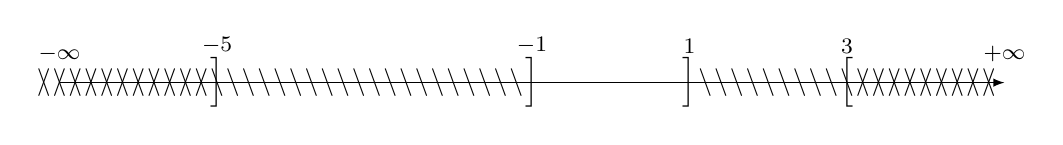
\begin{tikzpicture}[>=latex,scale=1]
%\draw (-7.5,-1) rectangle (5.5,1.5) ; 
% \clip (-1,-1) rectangle (5.5,2) ; 
    \draw[->] (-7,0) --(5,0);
    \node[] at (-5,0) {\bf $\Big]$};
    \node[] at (-1,0) {\bf $\Big]$};
    \node[] at ( 1,0) {\bf $\Big]$};
     \node[] at (3,0) {\bf $\Big[$};
    \node[above=4pt] at  (-7,0) {\footnotesize $-\infty$};
    \node[above=7pt] at  (-5,0) {\footnotesize $-5$};
    \node[above=7pt] at  (-1,0) {\footnotesize $-1$};
    \node[above=7pt] at  ( 1,0) {\footnotesize $1$};
    \node[above=7pt] at  ( 3,0) {\footnotesize $3$};
    \node[above=4pt] at  ( 5,0) {\footnotesize $+\infty$};
    \foreach \xp in {-7.2,-7,...,-5.2}{\node[] at(\xp,0) {$\slash$};}
    \foreach \xp in {-7.2,-7,...,-1.2}{\node[] at(\xp,0) {$\backslash$};}
    \foreach \xp in {1.2,1.4,...,4.8}{\node[] at (\xp,0) {$\backslash$};}
    \foreach \xp in {3.2,3.4,...,4.8}{\node[] at (\xp,0) {$\slash$};}
\end{tikzpicture}

\vspace*{.3cm}

D'où $S = \left]-1 \; ; \; 1\right]$. 

\newpage

\subsubsection{Exercice \no 3 : Un exemple de calcul de taux d'évolution moyen }

Entre 2002 et 2012, la dépense pour un élève de lycée a augmenté de $6,05\;$ \%. \\ 

Déterminer la valeur approchée à $10^{-2}$ près du taux annuel moyen de l'augmentation de la dépense. \\

Soit $D$ la dépense initiale. \\

\begin{tabular}{ll}
Taux réel : & $\! \! \! \! \!$ Dépense initiale $D$ \\
& $\! \! \! \! \!$ Dépense finale $D \times 1,0605$ \\
\end{tabular}

\vspace*{.3cm}

\begin{tabular}{lll}
Taux fictif : & Dépense initiale $D$ &  \\
& Dépense au bout & $\! \! \! \! \! \! \! \! \! \! \! \! \! \! \!$ d'un an : $D \times \left(1 + \dfrac{t}{100}\right)$ \\
& & $\! \! \! \! \! \! \! \! \! \! \! \! \! \! \!$ de deux ans : $D \times \left(1 + \dfrac{t}{100}\right)^2$ \\
& & $\! \! \! \! \! \! \! \! \! \! \! \! \! \! \!$ de trois ans : $D \times \left(1 + \dfrac{t}{100}\right)^2$ \\
& & $\! \! \! \! \! \! \! \! \! \! \! \! \! \! \!$ ... \\
& Dépense finale au & $\! \! \! \! \! \! \! \! \! \! \! \! \! $ bout de 10 ans : $D \times \left(1 + \dfrac{t}{100}\right)^{10}$ \\
\end{tabular}

\vspace*{.6cm}

\begin{tabular}{lll}
Ainsi $D \times 1,0605 = D \times \left(1 + \dfrac{t}{100}\right)^{10}$ & $\Longleftrightarrow$ & $1,0605 = \left(1 + \dfrac{t}{100}\right)^{10}$ \vspace*{.3cm} \\
& $\Longleftrightarrow$ & $\ln 1,0605 = \ln \left[\left(1 + \dfrac{t}{100}\right)^{10}\right]$ \vspace*{.3cm} \\
& $\Longleftrightarrow$ & $\ln 1,0605 = 10\ln \left(1 + \dfrac{t}{100}\right)$ \vspace*{.3cm} \\
& $\Longleftrightarrow$ & $\dfrac{1}{10} \times \ln 1,0605 = \ln \left(1 + \dfrac{t}{100}\right)$ \vspace*{.3cm} \\
& $\Longleftrightarrow$ & $e^{\frac{1}{10} \times \ln 1,0605} = 1 + \dfrac{t}{100}$ \vspace*{.3cm} \\
& $\Longleftrightarrow$ & $e^{\frac{1}{10} \times \ln 1,0605} - 1 = \dfrac{t}{100}$ \vspace*{.3cm} \\
& $\Longleftrightarrow$ & $t = 100\left(e^{\frac{1}{10} \times \ln 1,0605} - 1\right)$ \vspace*{.3cm} \\
\end{tabular}

On a $t \approx 0,59$. \\

Une augmentation de $6,05\; $ \% en 10 ans est équivalente à une augmentation annuelle \\ d'environ $0,59\;$ \% pendant 10 ans.

\newpage

\vspace*{-1.5cm}

\subsection{Exercices type Bac}

\subsubsection{Exercice Type Bac \no 1}

\begin{tabular}{llll}
Soit la fonction $f:$ & $\R$ & $\longrightarrow$ & $\R$ \\
& $x$ & $\longmapsto$ & $f(x) = e^{2x} + ae^x + b $ \\ \end{tabular}

\vspace*{.3cm}

On donne : \\

\variations
x & -\infty & & \ln 3 & & +\infty \\
f'(x) & &  & \z &  & \\
f(x) & \h{-7} & \dl & \b{ } & \cl & \h{ } \\
\fin

\vspace*{.3cm}

\begin{itemize}
\item[1.] Exprimer $f'(x)$ en fonction de $a$ et de $b$. \\
\item[2.]
\begin{itemize}
\item[a)] Déterminer $a$ et $b$ en utilisant le tableau de variations ci-dessus. 
\item[b)]  Déterminer $f\left(\ln 3\right)$ et $ \displaystyle {\lim_{x \rightarrow \infty}} \; f(x)$
\item[c)] Compléter le tableau de variations de $f$. \\
\end{itemize} 
\item[3.] Résoudre dans $\R$ :
\begin{itemize}
\item[a)] l'équation $e^{2x} - 6x - 7 = 16$ 
\item[b)] l'inéquation $e^{2x} - 6x - 7 \geqslant 16$ 
\end{itemize}
\end{itemize}

\vspace*{.3cm}

\begin{itemize}
\item[1.] $f$ est dérivable sur $\R$ et $f'$ est définie sur $\R$ par : $f'(x) = 2e^{2x} + ae^x$. \\
\item[2.]
\begin{itemize}
\item[a)] $\;$ • $\;$ Déterminer $a$ : \\
\end{itemize}
\end{itemize}

On sait que $f'\left(\ln 3\right) = 0$. \\

\begin{tabular}{lll}
D'où $2e^{2\ln 3} + ae^{\ln 3} = 0$ & $\Longleftrightarrow$ & $2e^{\ln\left(3^2\right)} + ae^{\ln 3} = 0$ \\
& $\Longleftrightarrow$ & $2e^{\ln 9} + ae^{\ln 3} = 0$ \\
& $\Longleftrightarrow$ & $2 \times 9 + 3a = 0$ \\
& $\Longleftrightarrow$ & $18 + 3a = 0$ \\
& $\Longleftrightarrow$ & $3a = -18$ \\
& $\Longleftrightarrow$ & $a = \dfrac{-18}{3}$ \\
& $\Longleftrightarrow$ & $a = -6$ \\
\end{tabular}

• Déterminer $b$ : \\

On sait que $ \displaystyle {\lim_{x \rightarrow -\infty}} \; f(x) = \displaystyle {\lim_{x \rightarrow -\infty}} \; \left(e^{2x} - 6x + b\right) = -7$. \\

Or, $\displaystyle {\lim_{x \rightarrow -\infty}} \; e^{2x} = 0$ et $\displaystyle {\lim_{x \rightarrow -\infty}} \; e^x = 0$. \\

D'où $b = -7$. \\

\begin{itemize}
\item[b)] $\;$ • $\;$ On calcule $f\left(\ln 3\right)$. \\
\end{itemize}

\begin{tabular}{lll}
$f\left(\ln 3\right)$ & $=$ & $e^{2\ln 3} - 6e^{\ln 3} - 7$ \\
& $=$ & $e^{\ln \left(3^2\right)} - 6e^{\ln 3} - 7$ \\
& $=$ & $e^{\ln 9} - 6e^{\ln 3} - 7$ \\
& $=$ & $9 - 3 \times 6 - 7$ \\
& $=$ & $9 - 18 - 7$ \\
& $=$ & $-16$ \\
\end{tabular}

\vspace*{-5cm}

\newpage

• On détermine $ \displaystyle {\lim_{x \rightarrow +\infty}} \; f(x)$. \\

$\displaystyle {\lim_{x \rightarrow +\infty}} \; f(x) = $ forme indéterminée, car $ \displaystyle {\lim_{x \rightarrow +\infty}} \; e^{2x} = +\infty $ et $ \displaystyle {\lim_{x \rightarrow +\infty}} \; e^x = +\infty $ \\

On peut lever l'indétermination en factorisant par $e^{2x}$ : \\

$f\left(x\right) = e^{2x} - 6e^x - 7 = e^{2x} \left(1 - \dfrac{6}{e^x} - \dfrac{7}{e^{2x}}\right)$. \\

$ \displaystyle {\lim_{x \rightarrow +\infty}} \; \left(1 - \dfrac{6}{e^x} - \dfrac{7}{e^{2x}}\right) = 1$, car $ \displaystyle {\lim_{x \rightarrow +\infty}} \; \dfrac{1}{e^x} = 0$ et $ \displaystyle {\lim_{x \rightarrow +\infty}} \;\dfrac{1}{e^{2x} = 0}$. \\

D'où $ \displaystyle {\lim_{x \rightarrow +\infty}} \; f(x) = +\infty$. \\

\begin{itemize}
\item[c)] On peut compléter le tableau de variations : \\
\end{itemize}

\variations
x & -\infty & & \ln 3 & & +\infty \\
f'(x) & & \color{red} - \color{black} & \z & \color{red} + \color{black} & \\
f(x) & \h{-7} & \dl & \color{red} \b{-16} \color{black} & \cl & \color{red} \h\pI \color{black} \\
\fin

\vspace*{.3cm}

\begin{itemize}
\item[3. a)] Résoudre dans $\R$ l'équation $e^{2x} - 6e^x - 7 = -16$. \\ 
\end{itemize}

\vspace*{.3cm}

$e^{2x} - 6e^x - 7 = -16 \Longleftrightarrow \left(e^x\right)^2 - 6e^x + 9 = 0$. \\

On pose $X = e^x$. \\

L'équation devient $X^2 - 6X + 9 = 0$ \\

\begin{tabular}{lll}
$X^2 - 6X + 9 = 0$ & $\Longleftrightarrow$ & $\left(X-3\right)^2 = 0$ \\
& $\Longleftrightarrow$ & $X -3 = 0$ \\
& $\Longleftrightarrow$ & $X = 3$ \\
& $\Longleftrightarrow$ & $e^x = 3$ \\
& $\Longleftrightarrow$ & $x = \ln 3$ \\
\end{tabular}

\vspace*{.3cm}

D'où $S = \lb \ln 3 \rb $ \\

\textbf{N.B. :} $x = \ln 3$ est une solution double. \\

\begin{itemize}
\item[b)] Résoudre dans $\R$ l'inéquation $e^{2x} - 6e^x - 7 \geqslant -16$. \\ 
\end{itemize}

\vspace*{.3cm}

$e^{2x} - 6e^x - 7 \geqslant -16 \Longleftrightarrow \left(e^x\right)^2 - 6e^x + 9 \geqslant 0$. \\

D'après la question $2)a)$, l'inéquation devient $\left(e^x - 3\right)^2 \geqslant 0$. \\

Or, un carré est toujours positif ou nul. \\

D'où $S = \left]-\infty \; ; \; +\infty\right[ = \R$.

\vspace*{-5cm}

\newpage

\vspace*{-2cm}

\subsubsection{Exercice Type Bac \no 2}

On considère la courbe donnée ci-dessous, représentative de la fonction $g$ définie et dérivable \\ sur l'intervalle $I = \left] 0 \; ; \; 21 \right]$. \\

La droite tracée sur le \hbox{graphique est la tangente à la courbe au point d'abscisse 1. Elle passe par l'origine.} \\

\begin{tabular}{ll}
\begin{minipage}{6cm}

\begin{itemize}
\item[1.] On note $g'$ la fonction dérivée de la fonction $g$ sur l'intervalle $I$. \\ Utiliser le graphique pour donner les valeurs de $g(1)$ et de $g'(1)$. \\
\item[2.]  On admet que pour tout $x$ de l'intervalle $I$, $g(x) = -4 + ax\left(3-b\ln x\right)$, où $a$ et $b$ sont deux nombres réels. \\ On veut calculer $a$ et $b$. \\
\begin{itemize}
\item[a)] Déterminer $g'(x)$.
\item[b)] À l'aide des valeurs de $g(1)$ et de $g'(1)$ obtenues à la question 1., calculer $a$ et $b$.
\end{itemize}
\end{itemize}
\end{minipage}
&
\begin{minipage}{9cm}
\begin{tikzpicture}[line cap=round,line join=round,>=triangle 45,x=5mm,y=2mm,scale=.9]
\draw[->] (-0.5,0) -- (22,0);
\foreach \x in {1,5,10,15,20}
\draw[shift={(\x,0)}] (0pt,2pt) -- (0pt,-2pt)node[below] {\footnotesize $\x$};
\draw (21,0) node[above] {\footnotesize $x$};

\draw[->] (0,-5) -- (0,27);
\foreach \y in {1,5,10,15,20,25}
\draw[shift={(0,\y)}] (2pt,0pt) -- (-2pt,0pt) node[left] {\footnotesize $\y$};
\draw (0pt,-8pt) node[left] {\footnotesize $0$};
\draw (0,26) node[right] {\footnotesize $y$};

\clip(-1,-5) rectangle (21,28);

\draw[smooth,samples=100,domain=0.01:21] plot(\x,{-4+4*(\x)*(3-ln(\x))});
\draw[smooth,samples=100,domain=-1.5:2.8] plot(\x,{8*(\x)});

\draw  (1,8)-- ++(-1.5pt,-1.5pt) -- ++(3.0pt,3.0pt) ++(-3.0pt,0) -- ++(3.0pt,-3.0pt);


\begin{pgfonlayer}{background}   
\draw[step=1mm,ultra thin,AntiqueWhite!10] (-1,-5) grid (22,28);
\draw[step=5mm,very thin,AntiqueWhite!30]  (-1,-5) grid (22,28);
\draw[step=1cm,very thin,AntiqueWhite!50]  (-1,-5) grid (22,28);
\draw[step=5cm,thin,AntiqueWhite]          (-1,-5) grid (22,28);
\end{pgfonlayer}

\end{tikzpicture}
\end{minipage}
\\
\end{tabular}

\vspace*{.3cm}

1. Graphiquement, on lit $g\left(1\right) = 8$ et $g'\left(1\right) = 8$. \\

\textbf{N.B. : } $g'(1)$ est le coefficient directeur de la droite tangente à la représentation graphique de $g$ \\ au point d'abscisse $1$. \\

On sait que $g(1) = 8$ et que la droite passe par l'origine, $g'(1) = \dfrac{y_A - y_0}{x_A - x_0} = \dfrac{8 - 0}{1 - 0} = 8$. \\

\begin{tabular}{lllll}
2.a) & $\! \! \! \! \! \! \! \! \! \! $ On pose & $u(x) = ax$ & et &  $v(x) = 3 - b\ln x$. \\
& $\! \! \! \! \! \! \! \! \! \! $ D'où & $u'(x) = a$ & et & $v'(x) = -b\times \dfrac{1}{x}$. \\
\end{tabular}

\vspace*{.3cm}

La fonction $g$ est de la forme $g = -4 + uv$. \\
On rappelle que la dérivée d'une constante est nulle, donc la dérivée de $g$ est \\ de la forme $g' = u'v + uv'$. \\

\begin{tabular}{lll}
D'où $\forall x \in I, g'(x)$ & $=$ & $a\left(3 - b\ln x\right) + ax \left(-b\times \dfrac{1}{x}\right)$ \vspace*{.3cm} \\
& $=$ & $3a - ab\ln x + ax \times \left(\dfrac{-b}{x}\right)$ \vspace*{.3cm} \\
& $=$ & $3a - ab\ln x - ab$ \\
\end{tabular}

\vspace*{.3cm}

b) On a $g(1) = 8$, d'où : \\

\begin{tabular}{lll}
$g(1) = 8$ & $\Longleftrightarrow$ & $-4 + a\times 1\left(3-\ln 1\right) = 8$ \\
& $\Longleftrightarrow$ & $a\left(3 - \ln 1\right) = 12$ \\
& $\Longleftrightarrow$ & $3a = 12$ \\
& $\Longleftrightarrow$ & $a = 4$ \\
\end{tabular}

\vspace*{.3cm}

On a $g'(1) = 8$, d'où : \\

\begin{tabular}{lll}
$g'(1) = 8$ & $\Longleftrightarrow$ & $3 \times 4 - 4b \ln 1 - 4b = 8$ \\
& $\Longleftrightarrow$ & $12 - 4b = 8$ \\
& $\Longleftrightarrow$ & $-4b = -4$ \\
& $\Longleftrightarrow$ & $b = 1$ 
\end{tabular}

\vspace*{-5cm}

\newpage

\subsubsection{Exercice Type Bac \no 3}

Le plan est rapporté à un repère orthogonal. \\

On désigne par $a$, $b$ et $c$ trois réels, et on considère la fonction $f$ définie sur $\left[0 \; ; \; 4\right]$ par : \\ $f(x) = ax^2 + bx + c$, dont on donne ci-dessous la représentation graphique $\Gamma$. \\

Les points $A$ et $B$ sont deux point de $\Gamma$. \\

La tangente à la courbe $\Gamma$ au point $A$ passe par le point $E\left(0 \; ; \; -1\right)$. \\

\begin{tikzpicture}[line cap=round,line join=round,>=triangle 45,x=2cm,y=1cm,scale=.8]
\draw[->] (-1.5,0) -- (4.2,0);
\foreach \x in {-1,1,2,3,4}
\draw[shift={(\x,0)}] (0pt,2pt) -- (0pt,-2pt)node[below] {\footnotesize $\x$};
\draw (4.2,0) node[above] {\footnotesize $x$};

\draw[->] (0,-6) -- (0,5.5);
\foreach \y in {-6,-5,-4,-3,-2,-1,1,2,3,4,5}
\draw[shift={(0,\y)}] (2pt,0pt) -- (-2pt,0pt) node[left] {\footnotesize $\y$};
\draw (0pt,-8pt) node[left] {\footnotesize $0$};
\draw (0,5.2) node[right] {\footnotesize $y$};

\clip(-1,-7) rectangle (4.5,6);

\draw[smooth,samples=100,domain=-1:5] plot(\x,{-2*(\x)*(\x) +7*(\x) -3});
\draw  (1,2)   node [right] {\footnotesize $A$} -- ++(-1.5pt,-1.5pt) -- ++(3.0pt,3.0pt) ++(-3.0pt,0) -- ++(3.0pt,-3.0pt);
\draw  (2,3)  -- ++(-1.5pt,-1.5pt) -- ++(3.0pt,3.0pt) node [right] {\footnotesize $B$}++(-3.0pt,0) -- ++(3.0pt,-3.0pt);
\draw  (0,-1) node [right] {\footnotesize $E$} ; % -- ++(-1.5pt,-1.5pt) -- ++(3.0pt,3.0pt) ++(-3.0pt,0) -- ++(3.0pt,-3.0pt);

\draw[smooth,samples=100,domain=-1.5:2.8] plot(\x,{-1+3*(\x)});



% \draw  (1,8)-- ++(-1.5pt,-1.5pt) -- ++(3.0pt,3.0pt) ++(-3.0pt,0) -- ++(3.0pt,-3.0pt);


\begin{pgfonlayer}{background}   
\draw[step=1mm,ultra thin,AntiqueWhite!10] (-1.5,-7) grid (4.5,6);
\draw[step=5mm,very thin,AntiqueWhite!30]  (-1.5,-7) grid (4.5,6);
\draw[step=1cm,very thin,AntiqueWhite!50]  (-1.5,-7) grid (4.5,6);
\draw[step=5cm,thin,AntiqueWhite]          (-1.5,-7) grid (4.5,6);
\end{pgfonlayer}

\end{tikzpicture}

\vspace*{.3cm}

\begin{itemize}
\item[1.] À l'aide du graphique : \\
\begin{itemize}
\item[a)] Donner l'image par $f$ de $1$, puis l'image par $f$ de $2$. 
\item[b)] Donner la valeur de $f'(1)$. \\
\end{itemize}
\item[2.] Déterminer les trois réels $a$, $b$ et $c$ à l'aide des résultats précédents. \\
\item[3.] Soit la fonction $g$ définie par $g(x) = \ln \left(-2x^2 + 7x - 3\right)$. \\
\begin{itemize}
\item[a)] Déterminer l'ensemble de définition $I$ de $g$. \\ Comment peut-on vérifier graphiquement ce résultats à l'aide de $\Gamma$ ?
\item[b)] Déterminer $g'(x)$ et résoudre l'équation $g'(x) = 0$.
\item[c)] Déterminer les limites de $f$ aux bornes de son ensemble de définition. 
\item[d)] Dresser le tableau de variations de la fonction $g$.
\end{itemize}
\end{itemize}

\newpage

\begin{itemize}
\item[1.]
\begin{itemize}
\item[a)] Graphiquement, on lit $f(1) = 2$ et $f(2) = 3$. \\
\item[b] $f'(1) = \dfrac{y_A - y_E}{x_A - x_E} = \dfrac{2-\left(-1\right)}{1 - 0} = \dfrac{3}{1} = 3$ \\
\end{itemize}
\item[2.] On sait que $f(x) = ax^2 + bx + c$, d'où $f'(x) = ax + b$. \\
\end{itemize}

\begin{tabular}{llll}
D'après les résultats de la question 1, on a : & $f(1) = 2$ & $\Longleftrightarrow$ & $a + b + c = 2$ \\
& $f(2) = 3$ & $\Longleftrightarrow$ & $4a + 2b + c = 3$. \\
& $f'(1) = 3$ & $\Longleftrightarrow$ & $2a + b = 3$ \\
\end{tabular}

\vspace*{.3cm}

\begin{tabular}{llll}
Il vient : & $\left\{
  \begin{array}{rll}
    a + b + c & = & 2 \\
    4a + 2b + c & = & 3 \\
   2a + b & = & 3 \\
  \end{array}
\right.$
& $\Longleftrightarrow$ & 
$\left\{
  \begin{array}{rll}
    a + \left(3 - 2a\right) + c & = & 2 \\
    4a + 2\left(3 - 2a\right) + c & = & 3 \\
    b & = & 3 - 2a \\
  \end{array}
\right.$ \vspace*{.3cm} \\
$\Longleftrightarrow$ & 
$\left\{
  \begin{array}{rll}
    -a + 3 + c & = & 2 \\
    4a + 6 - 4a + c & = & 3 \\
    b & = & 3 - 2a \\
  \end{array}
\right.$
& $\Longleftrightarrow$ & 
$\left\{
  \begin{array}{rll}
    -a + c & = & -1 \\
    6 + c & = & 3 \\
    b & = & 3 - 2a \\
  \end{array}
\right.$ \vspace*{.3cm} \\
$\Longleftrightarrow$ & 
$\left\{
  \begin{array}{rll}
    -a + c & = & -1 \\
     c & = & -3 \\
    b & = & 3 - 2a \\
  \end{array}
\right.$ 
& $\Longleftrightarrow$ & 
$\left\{
  \begin{array}{rll}
    -a - 3 & = & -1 \\
     c & = & -3 \\
    b & = & 3 - 2a \\
  \end{array}
\right.$ \vspace*{.3cm} \\
$\Longleftrightarrow$ & 
$\left\{
  \begin{array}{rll}
    a + 3 & = & 1 \\
     c & = & -3 \\
    b & = & 3 - 2a \\
  \end{array}
\right.$
& $\Longleftrightarrow$ & 
$\left\{
  \begin{array}{rll}
    a & = & -2 \\
     c & = & -3 \\
    b & = & 3 - 2\times \left(-2\right) \\
  \end{array}
\right.$ \vspace*{.3cm} \\
$\Longleftrightarrow$ & 
$\left\{
  \begin{array}{rll}
    a & = & -2 \\
     c & = & -3 \\
    b & = & 3 + 4 \\
  \end{array}
\right.$ 
& $\Longleftrightarrow$ & 
$\left\{
  \begin{array}{rll}
    a & = & -2 \\
     c & = & -3 \\
    b & = & 7 \\
  \end{array}
\right.$ \\
\end{tabular}

\vspace*{.3cm}

D'où $f(x) = -2x^2 + 7x - 3$. \\

\begin{tabular}{lllll}
3. a) Soit la fonction $g:$ & $\R$ & $\longrightarrow$ & $\R$ & \\
& $x$ & $\longmapsto$ & $g(x)$ & $\! \! \! \! \! \! \! \! \!= \ln \left(-2x^2 + 7x - 3\right)$ \\
& & & & $\! \! \! \! \! \! \! \! \! = \ln\left[f\left(x\right)\right]$ \\
\end{tabular}

Il faut que $f(x) > 0$. \\

Graphiquement, on lit que $\Gamma$ est au-dessus de l'axe des abscisses sur l'intervalle $I = \left]\dfrac{1}{2} \; ; \; 3\right[$. \\

Donc graphiquement, on a $I = \left]\dfrac{1}{2} \; ; \; 3\right[$. \\

Par le calcul, on étudie le trinôme $-2x^2 + 7x - 3$. \\

\begin{tabular}{lll}
$\Delta$ & $=$ & $b^2 - 4ac$ \\
& $=$ & $49 - 4 \times \left(-2\right) \times \left(-3\right)$ \\
& $=$ & $49 - 24$ \\
& $=$ & $25$ \\
\end{tabular}

\newpage

\vspace*{-1.5cm}

$\Delta > 0$, donc le trinôme admet deux racines : \\

\begin{tabular}{lll}
$x_1 = \dfrac{-b - \sqrt{\Delta}}{2a}$ & et & $x_2 = \dfrac{-b + \sqrt{\Delta}}{2a}$ \vspace*{.3cm} \\
$x_1 = \dfrac{-7 - 5}{2\times \left(-2\right)}$ & et & $x_2 = \dfrac{-7 + 5}{2\times \left(-2\right)}$ \vspace*{.3cm} \\
$x_1 = \dfrac{-12}{-4}$ & et & $x_2 = \dfrac{-2}{-4}$ \vspace*{.3cm} \\
$x_1 = 3$ & et & $x_2 = \dfrac{1}{2}$ \\
\end{tabular}

\vspace*{.5cm}

On peut en déduire le tableau de signes suivant : \\

\begin{tikzpicture}
\tkzTabInit[lgt=5,espcl=2]
{ $x$               /1,
$-2x^2 + 7x - 3$     /1}
{$ - \infty $ , $\dfrac{1}{2}$, $3$, $+ \infty $}
\tkzTabLine{ , - , z , + , z , - , }
\end{tikzpicture}

\vspace*{.3cm}

D'où $I = \left]\dfrac{1}{2} \; ; \; 3\right[$. \\

\begin{itemize}
\item[b)] On admet que pour $u$ une fonction, on a $\left(\ln u\right)' = \dfrac{u'}{u}$. \vspace*{.3cm} \\
\end{itemize}

D'où $g'(x) = \dfrac{-4x + 7}{-2x^2 + 7x - 3}$. \\

On résout ensuite l'équation $g'(x) = 0$. \\

\begin{tabular}{lll}
$g'(x) = 0$ & $\Longleftrightarrow$ & $\dfrac{-4x + 7}{-2x^2 + 7x - 3} = 0$ \vspace*{.3cm} \\
& $\Longleftrightarrow$ & $-4x + 7 = 0$ \vspace*{.3cm} \\
& $\Longleftrightarrow$ & $-4x = -7$ \vspace*{.3cm} \\
& $\Longleftrightarrow$ & $x = \dfrac{7}{4}$  \\ 
\end{tabular}

\vspace*{.3cm}

$\forall x \in \left]\dfrac{1}{2} \; ; \; 3\right[$, $-2x^2 + 7x - 3 > 0$, donc le signe de $g'(x)$ est de signe de $-4x + 7$. \\

\begin{itemize}
\item[c)] On a $\lim\limits_{\substack{x \to \frac{1}{2} \\ x>\frac{1}{2}}} \; g(x) = -\infty$ et $\lim\limits_{\substack{x \to 3 \\ x<3}} \; g(x) = -\infty$ \\
\end{itemize}

\textbf{N.B. : } On note aussi $ \displaystyle {\lim_{x \rightarrow \frac{1}{2}^+}} \; g(x) = -\infty$ et $ \displaystyle {\lim_{x \rightarrow 3^-}} \; g(x) = -\infty$. \\

\begin{itemize}
\item[d)] On peut donc dresser le tableau de signes de $g'(x)$ et en déduire les variations de $g$ : \\
\end{itemize}

\vspace*{.1cm}

\variations
x & -\infty & & \frac{1}{2} & & & \frac{7}{4} & & & 3 & & +\infty \\
g'(x) & \ha & \ha & \bb & &  + & \z & - & &  \bb & \ha & \ha \\
g(x) & \hv & \hv & \bb & \b\mI & \cl & \h{\ln \frac{7}{4}} & \dl & \b\mI &  \bb & \hv & \hv \\
\fin

\vspace*{.3cm}

$g$ admet un maximum absolu en $M\left( \dfrac{7}{4} \; ; \; \ln \dfrac{7}{4} \right)$.

\vspace*{-5cm} 